\documentclass[review]{elsarticle}
\usepackage{lineno,hyperref}
\modulolinenumbers[5]

\journal{Journal of Artificial Intelligence}

\usepackage[utf8]{inputenc}
\usepackage{amsmath}
\usepackage{relsize}
\usepackage{amssymb}
\numberwithin{equation}{section}
\usepackage{pdfpages}
\usepackage{caption}
\usepackage{subcaption}
\usepackage{fullpage}
\usepackage{xcolor,tabularx}
\usepackage{wrapfig}
\usepackage{hyperref}
\usepackage{placeins}

\usepackage{algorithm}
\usepackage[noend]{algpseudocode}
\usepackage{algorithmicx}
\usepackage[makeroom]{cancel}

\usepackage{float}

\newsavebox{\fmbox}
\newenvironment{fmpage}[1]
{\begin{lrbox}{\fmbox}\begin{minipage}{#1}}
{\end{minipage}\end{lrbox}\fbox{\usebox{\fmbox}}}

\DeclareMathOperator{\Tr}{Tr}
\DeclareCaptionLabelFormat{adja-page}{\hrulefill\\#1 #2 \emph{(previous page)}}

\usepackage{hyperref}
\hypersetup{
    colorlinks,
    citecolor=black,
    filecolor=black,
    linkcolor=black,
    urlcolor=black
}

\usepackage{tikz}
\usetikzlibrary{decorations.pathreplacing,calc}
\newcommand{\tikzmark}[1]{\tikz[overlay,remember picture] \node (#1) {};}

\newcommand*{\AddNote}[4]{%
    \begin{tikzpicture}[overlay, remember picture]
        \draw [decoration={brace,amplitude=0.5em},decorate,ultra thick,red]
            ($(#3)!(#1.north)!($(#3)-(0,1)$)$) --  
            ($(#3)!(#2.south)!($(#3)-(0,1)$)$)
                node [align=center, text width=2.5cm, pos=0.5, anchor=west] {#4};
    \end{tikzpicture}
}%


\newcommand\Ccancel[2][black]{\renewcommand\CancelColor{\color{#1}}\cancel{#2}}



\bibliographystyle{elsarticle-num}

\setlength\floatsep{1.25\baselineskip plus 3pt minus 2pt}
\setlength\textfloatsep{1.25\baselineskip plus 3pt minus 2pt}
\setlength\intextsep{1.25\baselineskip plus 3pt minus 2 pt}

\def\BState{\State\hskip-\ALG@thistlm}


\begin{document}


\newcommand{\V}{\ensuremath{\mathcal{V}}}
\newcommand{\varOne}{\ensuremath{\sigma_{x}^{2}}}
\newcommand{\varTwo}{\ensuremath{\sigma_{m}^{2}}}
\newcommand{\stdOne}{\ensuremath{\sigma_{x}}}
\newcommand{\stdTwo}{\ensuremath{\sigma_{m}}}
\newcommand\independent{\protect\mathpalette{\protect\independenT}{\perp}}\def\independenT#1#2{\mathrel{\rlap{$#1#2$}\mkern2mu{#1#2}}}
\newcommand{\dependent}{\rotatebox[origin=c]{180}{$\independent$}}

\newcommand{\BigO}[1]{\ensuremath{\operatorname{O}\bigl(#1\bigr)}}


\begin{frontmatter}

\title{Measurement Likelihood Memory for Bayesian State Estimation\\ for search scenarios}

\author{Guillaume de Chambrier and Aude Billard}
\address{Ecole Polytechnique Federale de Lausanne (EPFL), Route Cantonale, 1015 Lausanne, Switzerland}

\begin{abstract}

Simultaneous Localisation and Mapping (SLAM) is concerned with the development of filters to accurately and efficiently infer the state parameters
(position, orientation,...) of an agent and aspects of its environment, commonly referred to as the map. It is necessary for that the agent achieves situatedness 
which is a precondition planning and reasoning. In this work we consider an agent who is given the task of finding a set of objects.
The agent has limited perception and can only sense the presences of objects if a direct contact is made. 
In the absence of recurrent sightings or direct measurements of objects there are no correlations from the measurement errors which 
can be exploited. This renders SLAM estimators, for which this fact is their backbone, ineffective. 
No assumptions are taken with respect to the marginals (beliefs) of both the agent and feature-based.
This leads to additional restrictions on current SLAM methodologies for which the parametrisation of the agent's and object's joint distribution is a Multivariate Gaussian.
From the loose assumptions we stipulate regarding the marginals, we adopt a histogram parametrisation. 

We introduce a SLAM algorithm, which we name Measurement Likelihood Memory Filter (MLMF), in which the joint distribution is not parametrised  
but instead we directly apply changes from the filtering step to the marginals. 

This is achieved by keeping track of the history of measurement likelihood 
functions. We demonstrate that our approach gives the same filtered marginals as a histogram filter and show two implementations in which
both have linear space complexity with one showing an exponential time complexity (although an order of magnitude smaller
than the histogram filter) and the other showing a linear time complexity which we call scalable-MLMF. We further quantitatively  demonstrate 
the scalability of our algorithm with 25 beliefs having up to 10'000'000 states. In an Active-SLAM setting we evaluate the impact that the size of the 
memory's history has on the decision theoretic process in a search scenario for a one step look ahead information gain planner.
We report on both 1D and 2D experiments.
\end{abstract}

\begin{keyword}
SLAM, Bayesian State Estimation, Graphical Models
\end{keyword}

\end{frontmatter}
\newpage
\linenumbers

\section{Introduction}

% Introduction of SLAM
Estimating the location or state parameters of a mobile agent whilst simultaneously building a map of the environment has been
regarded as one of the most important problems to be solved for agents to achieve true autonomy. It is a necessary precondition for 
any agent to have at its disposal an estimation of the world which accurately encompasses all knowledge and their uncertainties. There has 
been a tremendous amount of research surrounding the field of Simultaneous Localisation And Mapping (SLAM) which branches out in a wide variety of sub-fields 
which deal with problems from building accurate noise models of the agent sensors \cite{Plagemann07gaussianbeam}, to determining which environmental 
feature was the cause of a particular measurement also known as the \textit{data association problem}\cite{DataAssociation2003} and many more. 

% Why does SLAM Work

Although the amount of research might seem overwhelming at first hand, all current SLAM methodologies are founded on a single principle; 
the uncertainty of the map is correlated through the agent's measurements. If the agent localises itself (by reducing position uncertainty)
all previously seen landmarks will also have their uncertainty reduced since the uncertainty is correlated with that of the agent's uncertainty.

% The three main pillar of SLAM algorithm and their respective draw backs

There are three main paradigms to solving the SLAM problem. The first is EKF-SLAM (Extendend-Kalman Filter)\cite{SLAM_part1}.
EKF-SLAM models the full state being the agent's parameters and environmental features by a Multivariate Gaussian distribution. 
The uncertainty of each individual feature is parametrised by a mean (expected position of the feature) and covariance 
(how much uncertainty there is about the position of the feature).

The second approach is Graph-SLAM\cite{TutGraphSLAM}. Graph-SLAM estimates the full path of the agent and considers every measurement to 
be a constraint on the agent's path. It is parametrised by the canonical Multivariate Gaussian. At each time step a new row and column 
is added to the precision matrix which encodes landmarks which have been observed as constraints on the robot's position.
At predetermined times, a nonlinear sparse optimisation is solved to minimise all the constraints on the robot's path which have been accumulated.

The third method is FastSLAM \cite{FastSLAM}. FastSLAM exploits the fact that if we know the position of the agent with 
certainty all landmarks become independent. It models the distribution of the agent's position by a particle filter. Each particle
has its own copy of the map and updates all landmarks independently of one another. The strength of this method is that the landmark
updates are simple since they are all independent. The draw back is that if many particles are required each must have its own copy of the map. 
It is beyond the scope of this paper to provide a detailed review of these  three paradigms and the reader is referred to \cite{Thrun_Burgard_Fox_2005}, \cite{SLAM_HBR}.

\paragraph*{Active-SLAM \& Exploration}

Active-SLAM refers to a decision theoretic process of choosing control actions so as to actively 
increase the convergence of the map. It is used in conjunction with exploration of an unknown environment
in a SLAM setting. The two steps of this process are: (i) generate a set of 
candidate destination positions, (ii) evaluate these positions based on a utility function. The utility  
is a trade off between reducing the uncertainty of the map or reducing the uncertainty
of the agent's position.

Most approaches use a two level representation of the map in an exploration setting. At the lower level
there is the chosen (landmark-based) SLAM filter and at the higher level a coarser representation of the world.
Such representations can be occupancy grids \cite{Thrun_grid_based_1996} which encode either occupied and free space
or a topological representation \cite{Kollar_2008_Exploration_SLAM}.

Early and current approaches to selecting candidate exploratory locations are based on evaluating 
Next-best-view \cite{Navigation_strategires_for_exploring_indoor_environments} locations. Next-best-view points are 
sampled around \textit{free edges} which are at the horizon of the known map (\textit{frontier} regions). 
In such a setting only target points are generated, not the full trajectory. Probabilistic Road Map (PRM) \cite{PRM_1996}
based methods have been used as planners to reach desired target locations, such as in \cite{RRT-SLAM}, where a Rapidly
Exploring Random Trees (RRT) is combined with FastSLAM. In \cite{ActivePosSLAM}, paths to \textit{frontier} regions are computed
via PRM  on a occupancy grid map and at the lower level they use Pose-SLAM (synonym for Graph-SLAM).

An alternative approach taken to generating candidate locations is the specification of high level macro actions, they being either 
\textit{exploratory} or \textit{revisiting} actions as is the case in \cite{stachniss05robotics}. The reason for the choice of macro actions is that the evaluation
of actions is costly, especially in the case of FastSLAM, since it requires propagating the filter 
forward in time so as to infer the information gain of each action.

The last approach is to solve the planning problem through formulating it as  Partially Observable Markov Decision Process (POMDP) \cite{Ross08onlineplanning}. 
However all methods take an approximation of the POMDP and consider a one time step planning horizon \cite[p.37]{GeorgiosLidoris}.

There are many ways of generating actions or paths, however their utility is nearly all exclusively based on the \textit{information gain}, 
which is the estimated reduction of entropy a particular action or path would achieve. A few utilities use f-measures such as the Kullback-Leibler divergence. 
Evaluation of different utility metrics are presented in \cite{Active_SLAM_Uncertainty_compar,tovar_planning,KL_SLAM_exploration_PF}.


\subsection{Problem Statement}

We consider an agent searching for a set of objects in a partially-known environment, in which exteroceptive feedback is extremely limited.
In the case of our agent, we can think of it as having a range sensor which only provides a response when in direct contact with an object. 
Our agent lives in a \textit{Table Top} world (see Figure \ref{fig:Figure1}) in which is located a set of objects.
The agent's uncertainty of its location and that of the objects is encoded by probability distributions $P(\cdot)$, which 
at initialisation are known as the agent's prior beliefs.

In Figure \ref{fig:Figure1} we illustrate a particular instance of the agent's beliefs about the world. 
The agent is currently located on the table and has only a vague idea of its location, somewhere about the centre right of the table. 
The scenarios considered are those in which there is a \textit{high level of uncertainty} as only environments to which the agent is not adapted are considered
and where the agent's perceptual capabilities are greatly reduced.

\begin{figure}
  \centering
  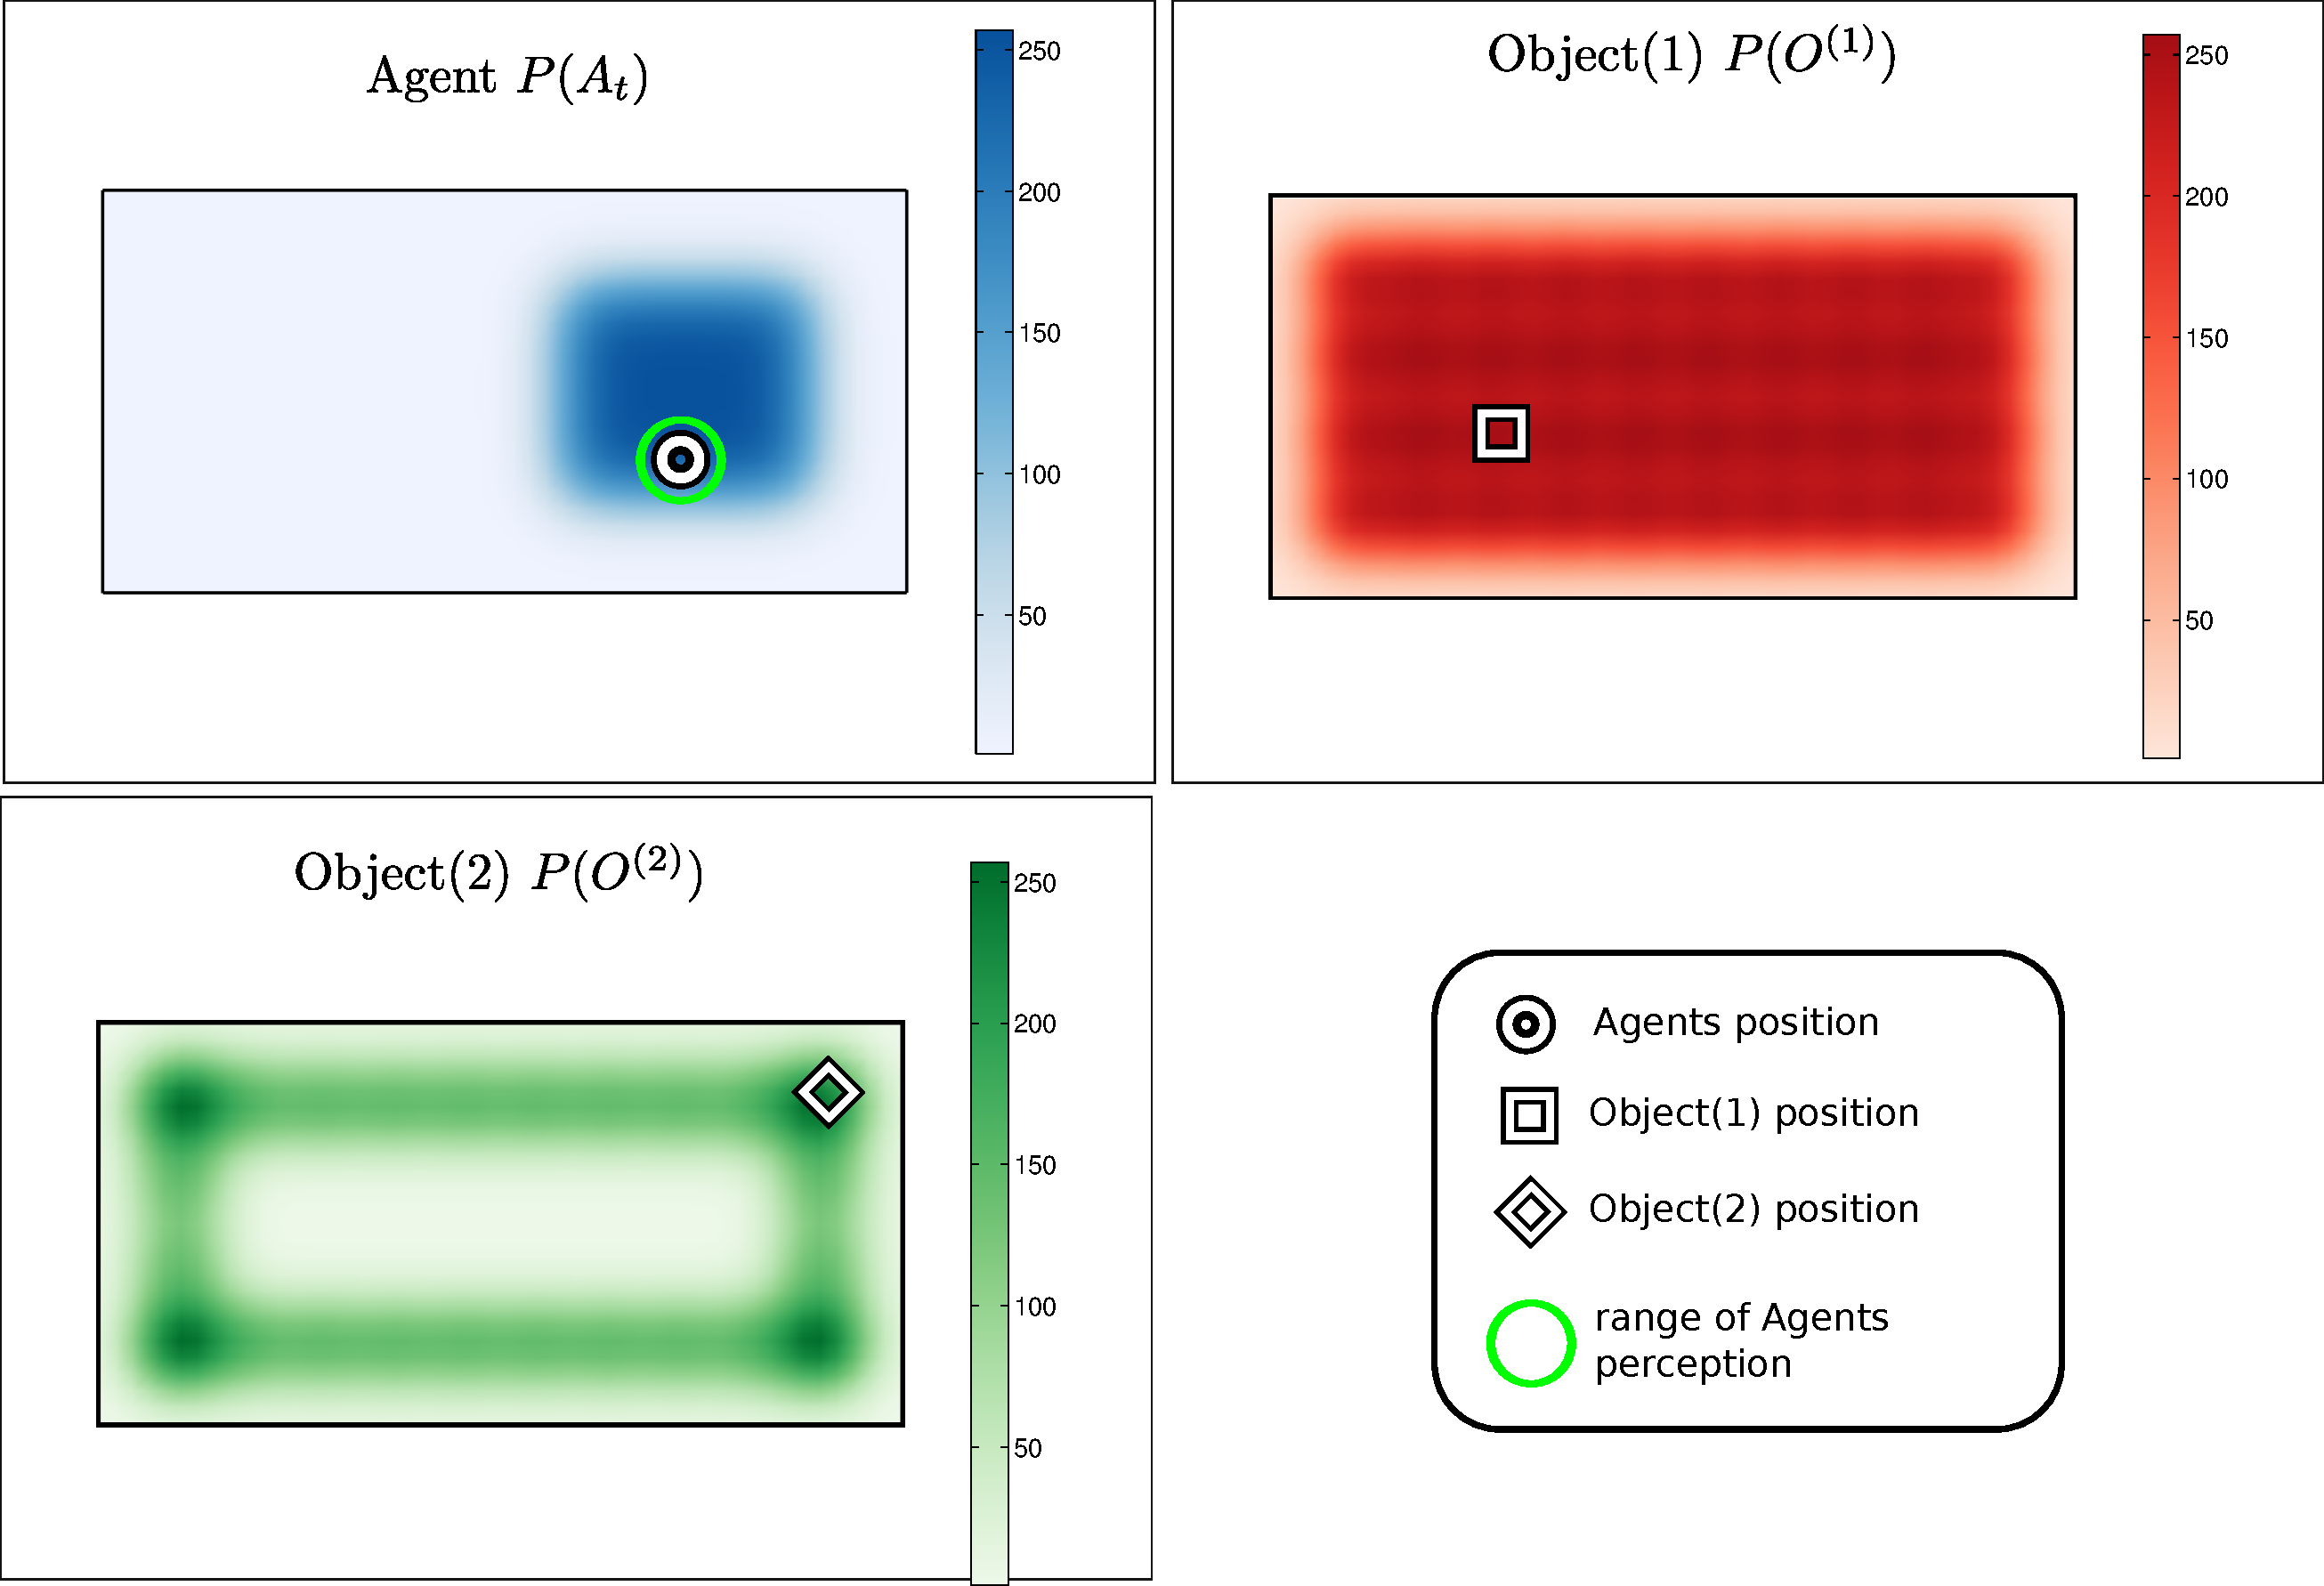
\includegraphics[width=0.95\linewidth]{Figure1.pdf}
  \caption{ \textit{Table Environment} Table Top World (delimited by the black rectangle), viewed from above, and the agent's beliefs. 
  There are three different probability density functions present on the table. 
  The blue represents the believed location of the agent, the red and green probability distributions are associated with object 1 and 2.
  The white shapes in each figure represent the true location of each associated object or agent.}
  \label{fig:Figure1}
\end{figure}
\vspace*{0.6cm}

%	2) Current draw back of all SLAM methodologies 
As the agent explores the world, it integrates all sensing information at each time step and updates its prior beliefs to posteriors
(the result of the prior belief after integrating motion and sensory information).
The main draw back of all current SLAM methods is that they only consider uncertainty induced by sensing inaccuracy inherent from 
the sensor and motion models. In our setting because of 
the limited range of the sensor we can confidently assume no measurement noise. 
In the scenario illustrated in Figure \ref{fig:Figure1}, the source of uncertainty is in the prior 
beliefs and the measurement information available to the agent is the 'absence of object' measurements. 
This is known as \textit{negative information} \cite[p.313]{Thrun_Burgard_Fox_2005}\cite{Thrun02particlefilters,negative_info_markov_localisation}. 
SLAM methodologies which use the error between the predicted and estimated position of the objects, such as in the case 
of EKF-SLAM and Graph-SLAM, will not work well in this setting. 

{\quote \textit{The EKF SLAM algorithm, [...], can only process positive sightings of landmarks. It cannot process negative information
that arises from the absence of landmarks. } (Probabilistic Robotics \cite[p.313]{Thrun_Burgard_Fox_2005})}

In addition to the negative sensing information, the original beliefs depicted in Figure \ref{fig:Figure1} are non-Gaussian
and multi-modal. We make no assumption regarding the form the beliefs can take. The implications are that no assumptions can be
made such that the joint distribution can be parametrised by a Multivariate Gaussian. This is an assumption made in many
SLAM algorithms, notably EKF-SLAM, and allows for a closed form solution to the state estimation problem. If the Gaussian assumption 
cannot be made then no closed form solution to the filtering problem is feasible. 
Using standard non-parametric methods (Kernel Density, Gaussian Process, Histogram,...) to represent or estimate the joint distribution becomes
unrealistic after a few dimensions or additional beliefs are added. 
FastSLAM would be a potential candidate, however because it parameterises the position uncertainty of the agent by a particle filter and each
particle has its own copy of the map the memory demand will become significant.  For planning purposes we would also want to have a 
single representation of the marginals.
Below we summarise the main aspects our filter should handle:\\[0.1cm]

\fbox{\parbox{0.9\textwidth-2\fboxsep-2\fboxrule}{%
\begin{itemize}
 \item Non-Gaussian joint distribution, no assumptions are made with respect to its form.
 \item Mostly negative information available (absence of positive sightings of the landmarks).
 \item Joint distribution volume grows exponentially with respect to the number of objects and states.
 \item Joint distribution volume is dense, there is a lot of uncertainty.
\end{itemize}
}}
\\[0.1cm]

\textit{The main contribution of our work and the importance to the field of Artificial Intelligence} 
An accurate estimate of the agent's belief space is a necessary precondition before planning or reasoning can be carried out.
In a wide range of Artificial Intelligence (AI) applications the agent's beliefs are discrete. This non-parametric representation
is the most unconstraining but comes at a cost. The parameterisation of the belief's joint distribution grows at the rate of a double exponential.
We propose a Bayesian state estimator which achieves the same filtered beliefs as a traditional filters but without the need to explicitly parametrise the state space 
of the joint distribution. Through memorising the measurement likelihood functions been applied on the joint distribution 
and by taking advantage of their structure, we achieve a filter which grows linearly as opposed to exponentially 
in both time and space complexity. We refer to our novel filter as the Measurement Likelihood Memory Filter (MLMF) because
of the fact that we keep track of the history of measurement likelihood functions, referred to as the memory, which 
have been applied on the joint distribution.
The MLMF filter allows to efficiently process negative information. To the authors knowledge there has been little
research on the integration of negative information in a SLAM setting. Previous work considered the case of active localisation \cite{NegInfoFurtherStudies}.
The incorporation of negative information is useful in many context and in particular in Bayesian Theory of Mind \cite{Bake_Saxe_Tene_2011}
where the reasoning process of a human is inferred from a Bayesian Network and in our own work \cite{deChambrier2013} were we model the search behaviour of a intentionally blinded
humans. In such a setting a lot of negative information is present and an efficient belief filter is required. Our work is thus applicable to the SLAM \& AI community in general
and the cognitive community which model human or agent behaviours through the usage of a Bayesian state estimators.


Through this new representation we implement a set of passive search trajectories through the state 
space and demonstrate, for a discretised state space, that our novel filter is optimal with respect to the Bayesian criteria (the successive
filtered posteriors are exact and not an approximate with respect to Bayes rule). We provide an analysis of the space and time complexity of 
our algorithm and prove that it is always more efficient under both criteria even when considering worst case scenarios.
Lastly we consider an Active-SLAM setting and evaluate the effect of how constraining the size of the number of memorised likelihood 
functions impacts the decision making process of a greedy one-step look-ahead planner.

\paragraph{Document structure}

The rest of the document is structured as follows: in section 2, we overview the Bayes filter recursion and apply it to a simple 
1D search scenario for both a discrete and Gaussian parametrisation of the beliefs. We demonstrate that discrete parametrisation gives
the correct filtered beliefs but at a very high cost and that the EKF-SLAM fails to provide the adequate solution. Section 3 we 
introduce the Measurement Likelihood Memory Filter and overview its parametrisation. Section 4 we derive the computational time and 
space complexity of the MLMF. Section 5 describes additional assumptions made with respect to the MLMF to make it 
scalable (scalable-MLMF). In section 6 we numerically evaluate the time complexity of the scalable-MLMF and check the assumption we made 
for it to be scalable. We investigate the filter's sensitivity with respect to its parameters in an Active-SLAM setting.



\section{Bayesian State Space Estimation}

The focus of Bayesian State Space Estimation (BSSE) is to incorporate observations or evidence to update a prior distribution over
the state space to a posterior distribution through the application of Bayes probability rules. The agent's random variable, $A$, 
is associated with the uncertainty of its location in the world, the same holds for the object(s') random variable(s), $O$. 
Given a sequence of actions and observations, $\{u_{1:t},y_{1:t}\}$ (subscript $1:t$ is the set from the time $t=1$ to the current time, $t=t$), 
algorithms of the BSSE family incorporate this information to provide an estimate $P(A_t,O|y_{1:t},u_{1:t})$. This is know as the 
filtering problem where all past information is incorporated to estimate the current state.  

\begin{figure}
\centering
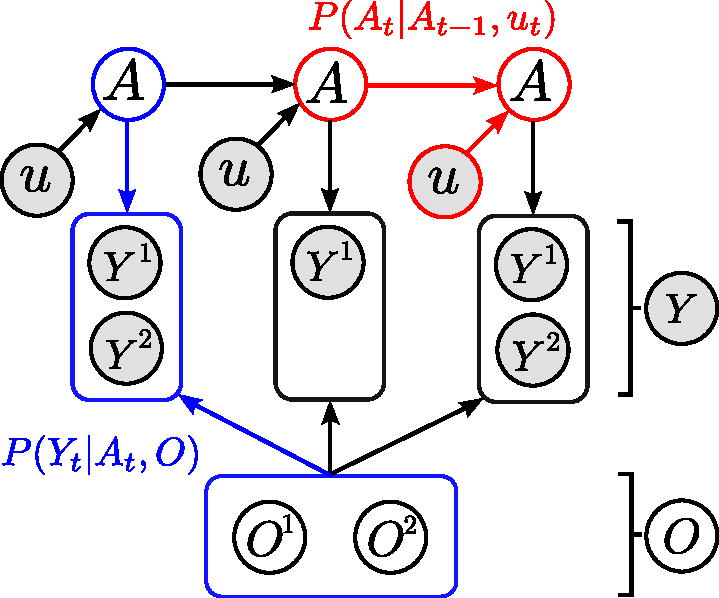
\includegraphics[width=0.4\textwidth]{Figure2.pdf}
\caption{Directed graphical model of dependencies between the agent(A), objects(O), sensing(Y) and action(u) random variables. Each 
object, $O^{(i)}$ is associated with one sensing random variable $Y^{(i)}$. The overall sensing random variable is $Y = \left[Y^{(1)},\dots,Y^{(M-1)}\right]^{\mathrm{T}}$,
where $M$ is the total number of agent and object random variables in the filter. 
For readability we have left out the time index $t$ from $A$ and $Y$. Since the objects are static, they have no temporal process associated with 
them thus they will never have a time subscript. The two models necessary for filtering are the motion model $P(A_t|A_{t-1},u_t)$ (red) and measurement model
$P(Y_t|A_t,O)$ (blue).}
\label{fig:bayesian_sse_dag}
\end{figure}

In Figure \ref{fig:bayesian_sse_dag} we depict the general Bayesian Network (BN) of a BSSE. The BN conveys two types of
information, the dependence and independence relations between the random variables in the graph which can be established
through \textit{d-separation} \cite{BayesBall}. The independence statements are the following: 1) $A_{t+1} \independent A_{t-1} | A_t$ the 
first order Markov property, 2) $A_{t} \independent Y_{t+1} | A_{t+1}$, past states do not depend on future observations, 
3) $A \independent O | \emptyset$ the agent and object random variables
are independent given no observation. The dependence statements of interest are: 1) $A \dependent O | Y$, which 
state that agent and object random variables will interact with each other given an observation. Any joint probability 
distribution whose factorisation  respects the structure of a BN is guaranteed to satisfy all the conditional independence 
statements which can be read from the graph. The converse with respect to the dependence statements is not guaranteed. There 
can be probabilistic dependencies which are present in the BN structure but not necessarily present in a chosen parametrisation 
of the joint probability distribution's factors \cite[p.43]{barberBRML2012}. This implies that BN are not suitable to model 
dependencies between random variables and are only suited to represent conditional independences. We demonstrate 
how the two different parametrisations of the joint distribution for the BN in Figure \ref{fig:bayesian_sse_dag} 
behave in the case of the absence of direct sighting of the object by the agent. Before this we review the steps necessary 
and models required for the Bayesian filtering problem.

\subsection{Bayesian filter}

The objective is to update the beliefs of the agent after every interaction with the environment. 
This can be obtained by recursively integrating \textit{motion} and \textit{measurements} into the joint distribution (equation \ref{eq:joint}).

\begin{equation}
 P(A_t,O|Y_{0:t},u_{0:t}) 
 \label{eq:joint}
\end{equation}

The general formulation of these two steps are provided below, see Appendix \ref{appendix:bayes_recursion} for complete derivation.

\paragraph{Motion-update:}
\begin{equation}\label{eq:time-update}
   P(A_t,O|Y_{0:t-1},u_{0:t}) = \sum_{A_{t-1}} P(A_t|A_{t-1},u_t) \cdot  P(A_{t-1},O_t|Y_{0:t-1},u_{0:t-1})
\end{equation}

\paragraph{Measurement-update:}
\begin{equation}\label{eq:measurement-update}
   P(A_t,O|Y_{0:t},u_{0:t}) = \frac{P(Y_t|A_t,O)\cdot P(A_t,O|Y_{0:t-1},u_{t}) }{P(Y_t|Y_{0:t-1})   }
\end{equation}

Two models are needed to perform the recursion, namely the motion model $P(A_t|A_{t-1},u_t)$ and the measurement model
$P(Y_t|A_t,O)$. We give an example for two different parametrisations of the distributions given above. In the first
case we consider the state space to be discrete, meaning that each conditional distribution will be parametrised by 
conditional probability tables (CPTs) and for the second case we look at the parametrisation used by EKF-SLAM. 


\subsubsection{Measurement model}\label{subsub:measurement-model}

\paragraph{Discrete CPTs measurement model}

A measurement model, $P(Y_t|A_t,O)$, should predict the likelihood of observations, $Y_t$, given the state of $A_t$ and $O$. 
In our case an observation is made only if the agent enters in contact with the object, which implies that both
occupy the same discrete state. If we were to discretise the state space to $N$ states, $x_i,\:i=1...N$, and the observation node $Y_t$  
has $M$ parents, then the size of the CPT table is $N^{M}$. In our case only the
entries for which both the agent and object are in the same state will have a probability of 1, all other entries will be 0.

\begin{align*}\label{eq:disc-measurement_function}
 P(Y_t=1|A_t=x_i,O=x_j) &= 1\;\; \forall i = j \\
 P(Y_t=1|A_t=x_i,O=x_j) &= 0\;\; \forall i \not= j \\
\end{align*}
 
\paragraph{EKF-SLAM measurement model}

The measurement model consists of two parts: the first part is the observation function, $h(\cdot)$, and the second part is the noise present in the measurement, 
typically always taken to be white Gaussian.

\begin{align}
  Y_t &= h(A_t,O) + \epsilon \\\nonumber
 \hat{Y}_t &= h(A_t,O)  
\end{align}

Where $Y_t$ is the actual current observation sensed by the agents sensors, $\hat{Y}_t$ is an estimated/predicted observation
and $\epsilon \sim \mathcal{N}(0,R)$ is the noise associated with the sensor measurement.
The measurement function returns the distance $r$ and bearing $\phi$ from the agent to an object, $Y = \left[r,\phi \right]^{\mathrm{T}}$. 
The limitation of the sensor range is governed by a radial basis function:
\begin{equation}\label{eq:ekf-measurement_function}
 h(x_i,x_j;\beta) = \exp\left(-\left( \beta \cdot \|x_i - x_j\| \right)^2 \right)
\end{equation}
Where $x_i$ and $x_j$ are the true locations of the agent and object. In EKF-SLAM these are taken to be the 
expectation of each random variable, $\mathbb{E}\{A_t\}$ and $\mathbb{E}\{O\}$. The larger the $\beta$, the smaller is the range of 
the sensor. The likelihood of an observation can be evaluated:
\begin{equation} \label{eq:lik-measurement}
   p(Y_t|A_t,O_t) = \frac{1}{|2\pi R|^{\frac{1}{2}}} \exp \left( -\frac{1}{2} \big(Y_t - \hat{Y}_t\big)^{\mathrm{T}}R^{-1}\big(Y_t - \hat{Y}_t\big) \right)
\end{equation}
Where the covariance, $R$, encompasses the uncertainty in the measurement. 

\subsubsection{Dynamic model}

\label{subsub:dynamic-model}
The dynamic model, in contrast to the measurement model, is much simpler. In our setting the model is a linear function of the 
current state and motor control, see Equation \ref{eq:dynamical_model}.

\begin{equation} \label{eq:dynamical_model}
  x_{t} = x_{t-1} + u_{t} + w \nonumber
\end{equation}

Where $w \sim \mathcal{N}(0,Q)$ is white Gaussian noise with mean zero and covariance $Q$. .

\subsection{Simultaneous Localisation and Mapping}

\subsubsection{Histogram/Discrete SLAM}\label{sec:Discrete}

In Figure \ref{fig:discrete_example} we demonstrate a simple 1D search in a discrete state space comprising 100 states. The joint
distribution table $P(A_t,O)$ is initialised to be the product of the two originally independent prior distributions of
the Agent and Object random variables $P(A_t)$ and $P(O)$. We then recursively apply the \textit{time} 
and \textit{measurement} update Equations \ref{eq:time-update} \& \ref{eq:measurement-update}.

\begin{figure}
\centering
  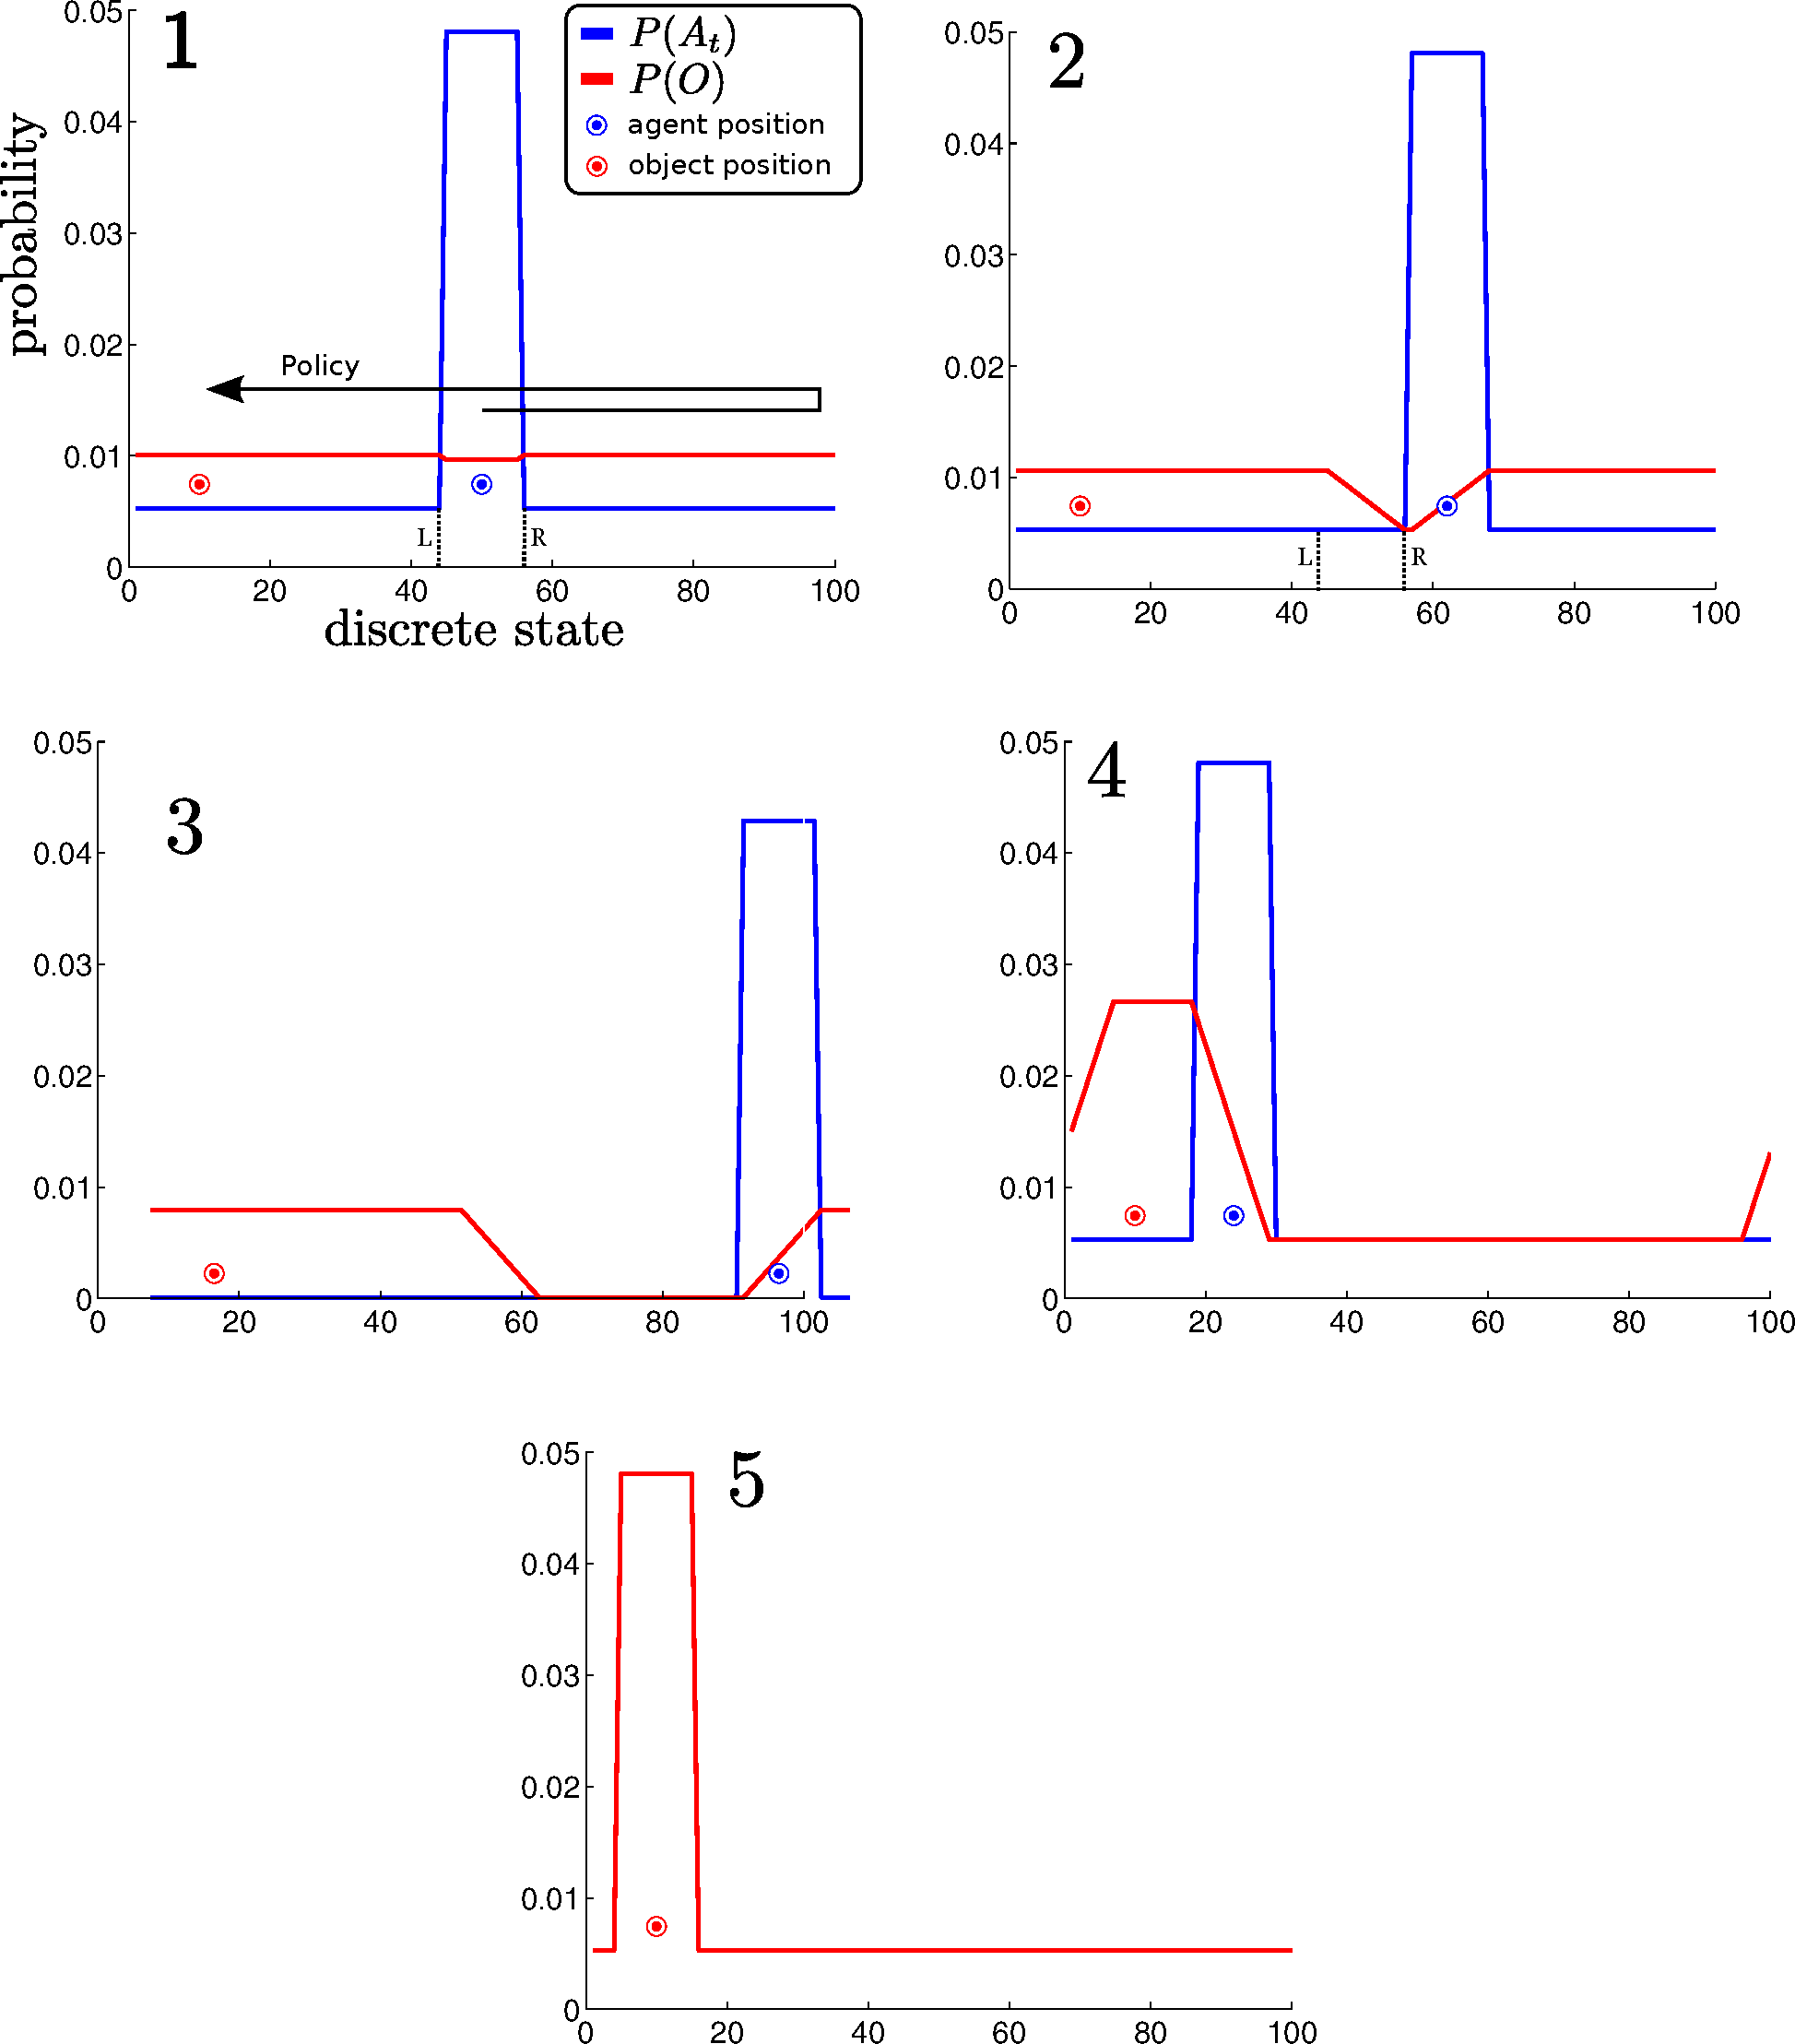
\includegraphics[width=0.8\textwidth]{Figure3.pdf}
 \caption{\textbf{Histogram SLAM} An agent and one object are present in the 1D world. The red and blue points represent the true
 locations whilst the lines are the probability of their current location (beliefs).
 (1) Initial beliefs, the marginals $P(A_t)$ and $P(O)$.
 The dotted lines annotated by L and R denote the left and right edges of the agent's belief mode. The agent will follow the policy
 shown by the black arrow which is a sweep to the right followed by one to the left.
 2) The left end of the agent's distribution has reached the initial right end of the distribution, see dotted lines for reference. When the left end, L,
 has reached the right end, R, the probability of the object being at R is equal to the underlying or ground uncertainty of the agent's belief. 
 From (3) to (4) object belief continuously increases in states 0 to 45.
 (5) agent and Object occupy the same state, the beliefs merge.}
 \label{fig:discrete_example}
\end{figure}

The search which was illustrated in Figure \ref{fig:discrete_example} gives the desired belief update, but at a significant cost, as the 
space complexity of the joint distribution is exponential in the number of beliefs. Given $M$ beliefs with
a total of $N$ states, the joint distribution will require $N^M$ parameters as will the conditional observation CPT table
$p(Y_t|A_t,O)$. 

\subsubsection{EKF-SLAM}\label{sec:EKF-SLAM}

In EKF-SLAM the joint distribution $p(A_{t},O|Y_{0:t},u_{0:t}) = g(x;\mu_t,\Sigma_t)$ is parametrised by a single Gaussian function $g$ with mean,
$\mu_t = \left[\mu_{A_{t}},\mu_{O^{(1)}},\dots,\mu_{O^{(M-1)}}\right]^{\mathrm{T}} \in \mathbb{R}^{3 + 2\cdot (M-1)}$  where the random variables 
are in $\mathbb{R}^2$, and covariance, $\Sigma_t$. 

\begin{equation}
\Sigma_t = \begin{bmatrix}
       \Sigma_a & \Sigma_{ao}  \\[0.3em]
       \Sigma_{oa} & \Sigma_o
     \end{bmatrix}
     \in \mathbb{R}^{(3 + 2\cdot (M-1)) \times (3 + 2\cdot (M-1))}
\end{equation}

The elements of the covariance matrix capture the measurement error between the true $Y$ and expected $\hat{Y}$ 
positions of the random variables. Because the joint distribution is parametrised by a single Multivariate Gaussian a closed 
form solution to the filtering Equations \ref{eq:time-update} \& \ref{eq:measurement-update} is possible and is given below:

\paragraph{Motion update}
\begin{align}
  \bar{\mu}_t      &= f(\mu_{t-1},u_t)\\
  \bar{\Sigma}_{t} &= F \Sigma_{t-1} F^{\mathrm{T}} + Q
\end{align}
Where $F = \left[\frac{\partial f(\mu_{t-1},u_t)}{\partial \mu_{t-1} } \right]$ is the Jacobian of the dynamic model with respect to the Gaussian mean. The 
bar notation on the mean and covariance is to indicate that no sensing information has been used to update their estimates.

\paragraph{Measurement update}

\begin{align}
   K    &= \bar{\Sigma}_{t} H (H \bar{\Sigma}_{t} H + R)^{-1} \\
  \mu_t &= \bar{\mu}_t + K \cdot (Y_t - \hat{Y}_t)\\
  \Sigma_t &= (I - KH) \bar{\Sigma}_{t}
\end{align}
 
Where $H = \left[\frac{\partial h(\mu_A,\mu_O;\beta)}{\partial \mu_A\mu_O}\right]$ is the Jacobian of the measurement function (Equation \ref{eq:ekf-measurement_function})  
with respect to the mean of the joint distribution. 

An important part in the application of EKF-SLAM is the error between the true measurement and the expected measurement 
$e = (Y_t - \hat{Y}_t)$. In our scenario the agent can only perceive the objects once he enters in direct contact with them. 
This means that the variance of the observation $Y_t$ will be very low and will always be equal to that of $\hat{Y}$ until a contact is made. To illustrate the problems this will
entail, we give an illustration of a 1D search as we did for the discrete case. In Figure \ref{fig:EKF-SLAM} we show the resulting updates of the belief 
for 4 chosen time segments.

\begin{figure}
\centering
\begin{subfigure}[t]{0.4\textwidth}
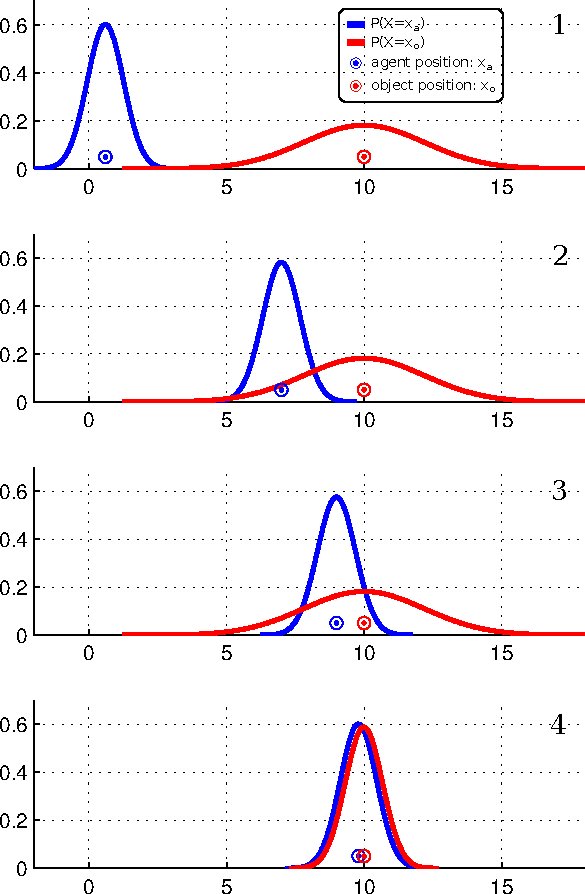
\includegraphics[width=\textwidth]{Figure4.pdf}

\caption{Time slices of the evolution of the pdfs according to EKF-SLAM. The numbers in the top right corner of each plot indicate the temporal ordering.
The blue pdf represents the agent's believed location and the circle with the dot in the middle is the true location of the agent. The same holds 
for the red distribution which represents the agent's belief of the location of an object.}

\label{fig:slam}
\end{subfigure}\qquad
\begin{subfigure}[t]{0.5\textwidth}
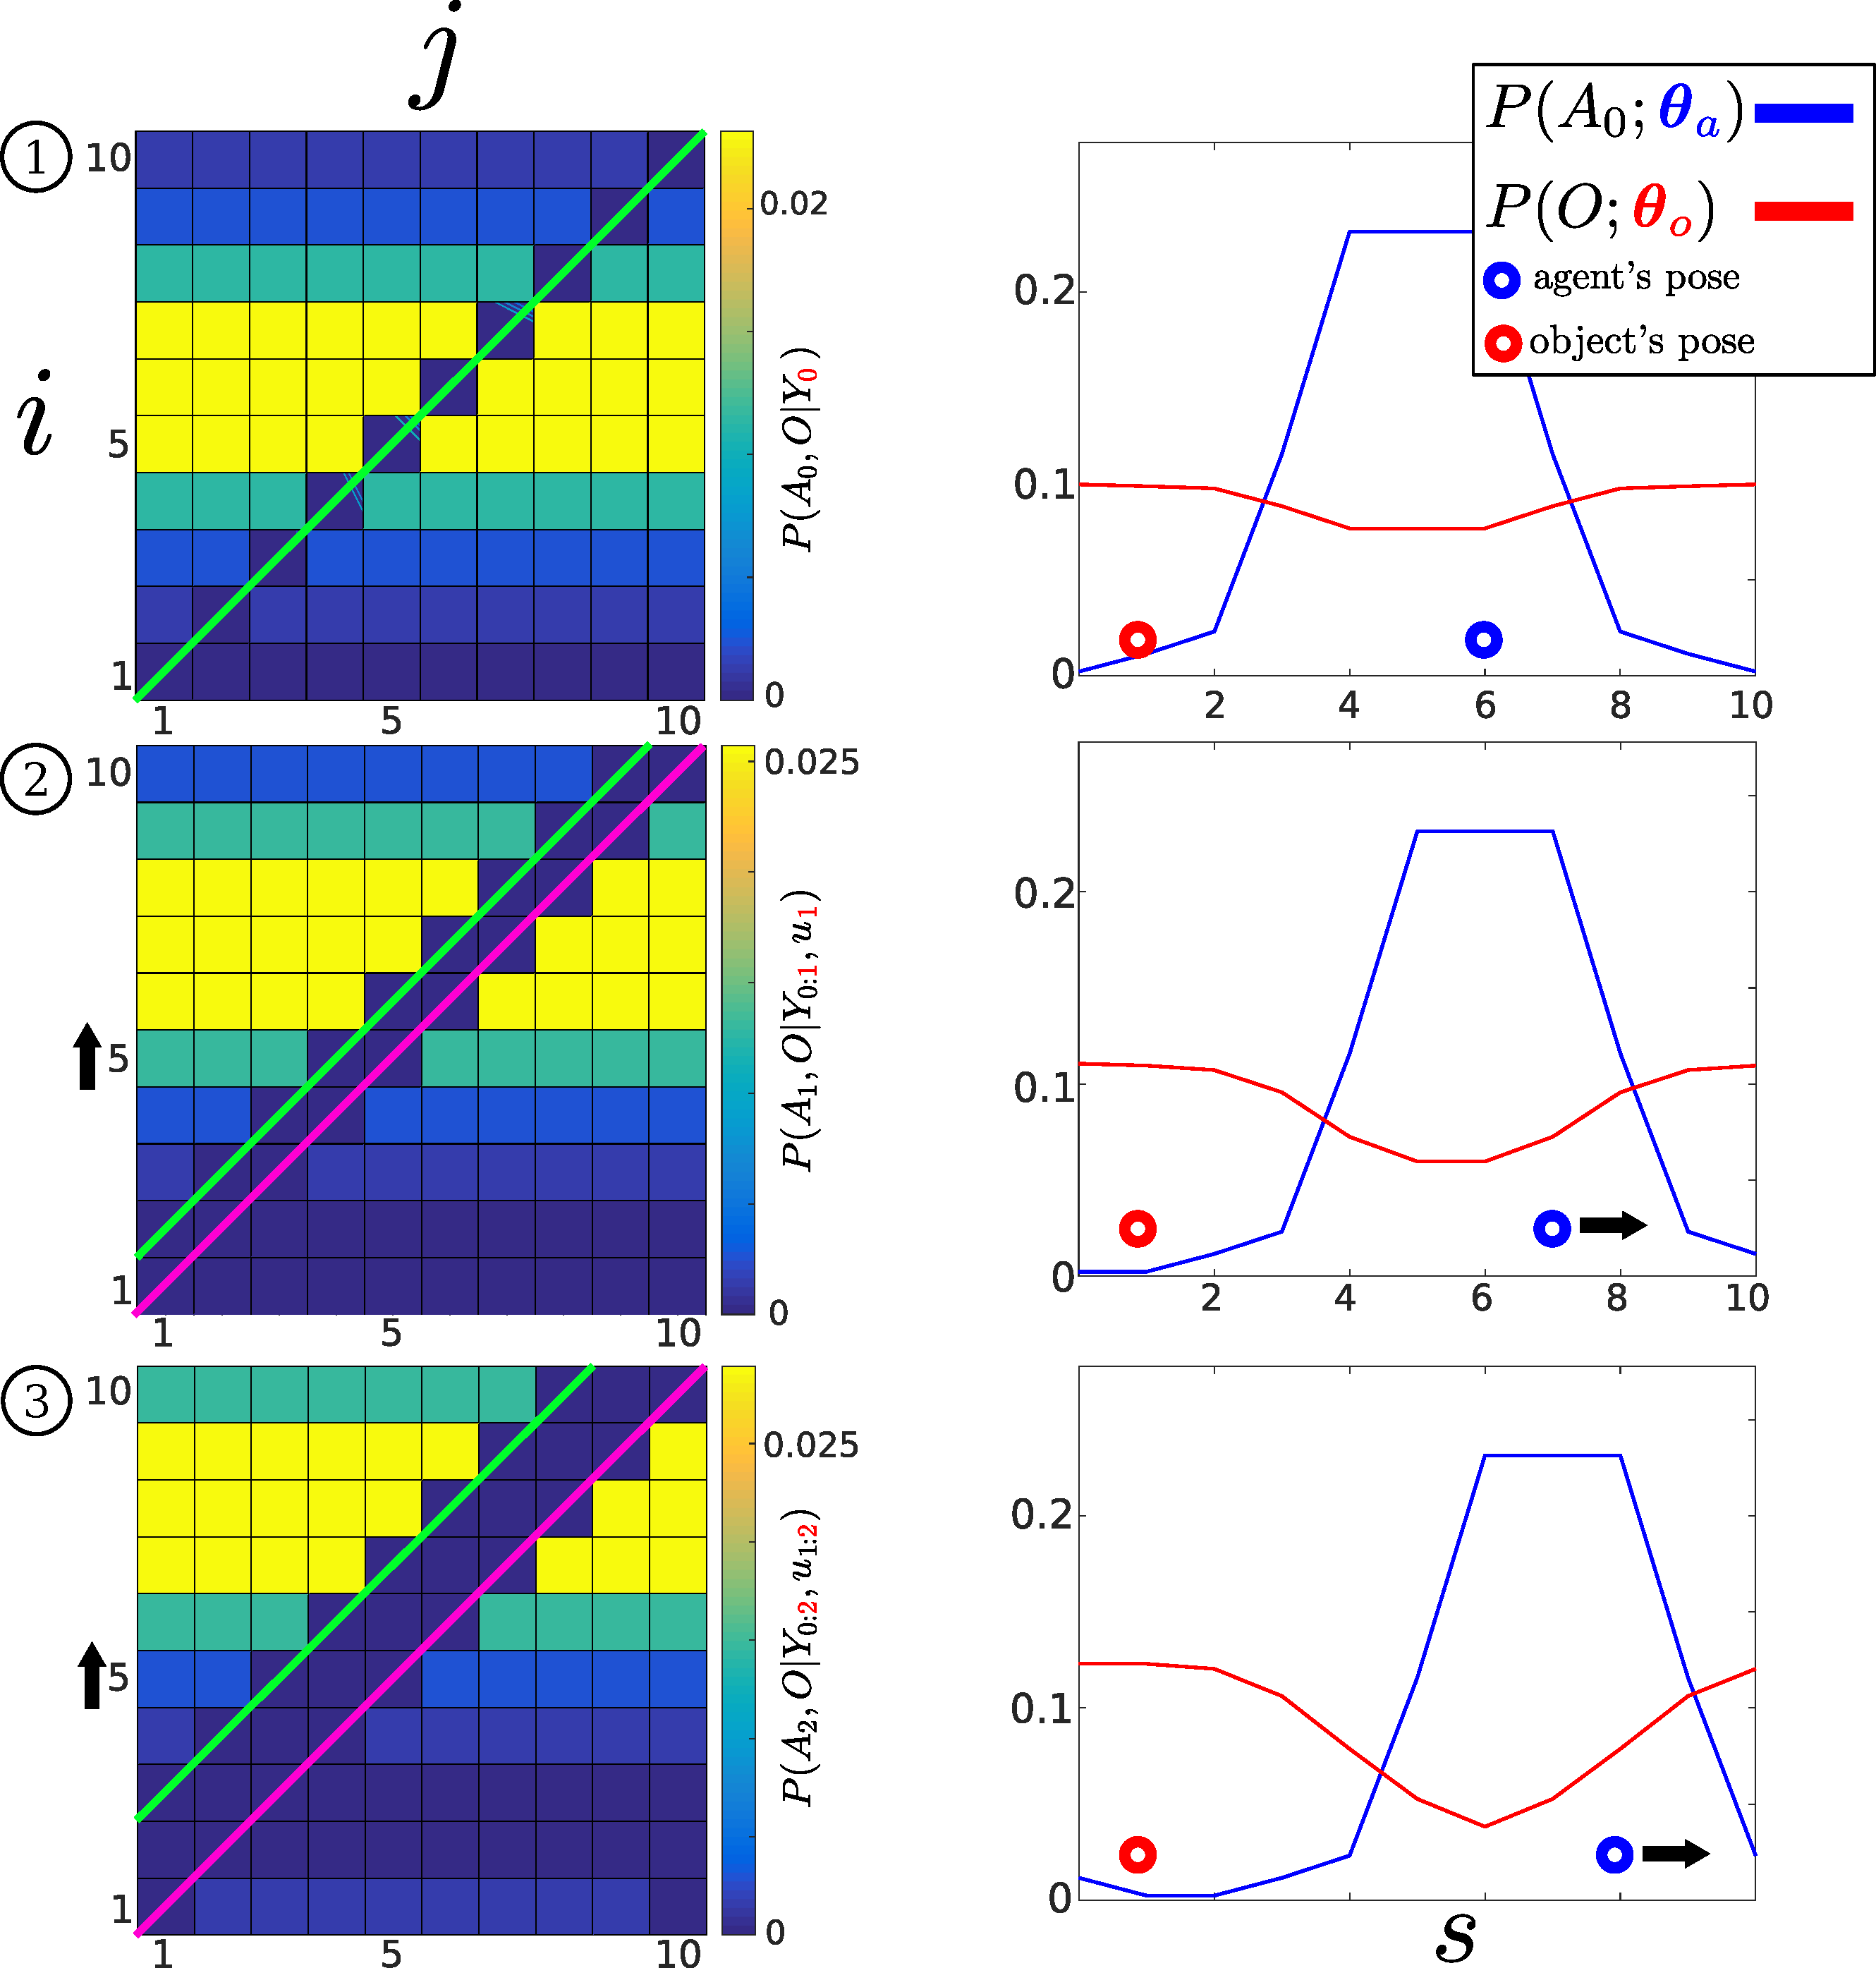
\includegraphics[width=\textwidth]{Figure5.pdf}

\caption{\textit{Top:} evolution of the Kalman gain, $K$, parameter according to the measurement error $e$. $K_a$ is the gain update for the 
agent's Gaussian parameters and $K_o$ is the gain update for the object. \textit{Middle:} evolution of the covariance components of 
$\Sigma$ over time. $\Sigma_a$ and $\Sigma_o$ are the variances of the agent and object positions and $\Sigma_{ao}$ is the cross covariance 
term. \textit{Bottom:} true sensing $Y_t$ and the expected sensation $\hat{Y}_t$.}

\label{fig:slam-para}
\end{subfigure}

\caption{1D EKF-SLAM, the figures to the left show the evolution of the agent's belief of his location and that of an 
object which are represented by the blue and red Gaussian functions. The figures to the right show the evolution of the parameters of the EKF-SLAM.}
\label{fig:EKF-SLAM}
\end{figure}

As expected we do not get the desired behaviour. Even when most of the belief mass of the agent's 
location pdf overlaps that of the object pdf, no belief update occurs. The chosen parametrisation of the BN for EKF-SLAM only guarantees a 
dependency between the agent and object random variables when there is a positive sighting of the landmarks:
$A \dependent O | Y$ iff $Y \not= 0$.  This can been seen in Figure \ref{fig:EKF-SLAM} (b), where the component 
$\Sigma_{ao}$ is 0 most of the time which implies that $A \independent O | Y$ which is undesirable. 
This confirms that the dependencies present in the structure given by the BN are dependent on the chosen parametrisation.


\FloatBarrier
\section{Measurement Likelihood Memory Filter}

To get the correct marginals' update, the random variables $A$ and $O$ must remain 
dependent in the absence of a positive observation $Y$ and in addition this dependence should be efficiently encoded in contrast to the
discrete/histogram parametrisation of the marginals of the joint distribution shown in Section \ref{sec:Discrete}. 

The measurement function $P(Y_t|A_t,O)$ is the cause of the dependence between the random variables. If both the agent and object 
where completely independent, no additional parameters would be required to represent the joint distribution other than the marginals 
$P(A_t)$ and $P(O)$ giving a total of $N \cdot M$ parameters ($N$ is the number of states and $M$ is the number of random variables). 
At the other extreme if every single point in the domain of the random variables was dependent this would require the totality 
of $N^M$ parameters as previously stated in the case of the histogram filter. We propose a method in which we do not model the joint
distribution explicitly but rather only compute its impact on the marginals. 

\subsection{New joint parametrisation \& intuition}

Figure \ref{fig:margina_joint_example} shows two time slices of the evolution of the agent and object belief in a 1D world. In the \textit{left}
figure a line passes through the probability mass of the joint distribution which was initialised to be independent,
$P(A_0,O) = P(A_0) \cdot P(O)$. 
This is the effect the measurement function $P(Y_t=0|A_t,O)$ has on the joint distribution given no object was sensed. As the agent 
moves towards state 100 the likelihood function is re-applied at every iteration and the result is visible in the \textit{right} figure. 
As a result the probability mass is removed from the area in the joint distribution where $P(Y_t=0|A_t,O)$ has an influence.
Because of the structure of the measurement likelihood function, this will always be on the $A=0$ axis in the joint distribution. 
The same is true for a range and bearing measurement function where the range translates to the width of the tube created in the 
joint distribution. Our method will rely on remembering the applied measurement function on the joint distribution rather than the result. 
It is far more efficient to remember a function than the values it changed in the
joint distribution.

\begin{figure}
 \centering
 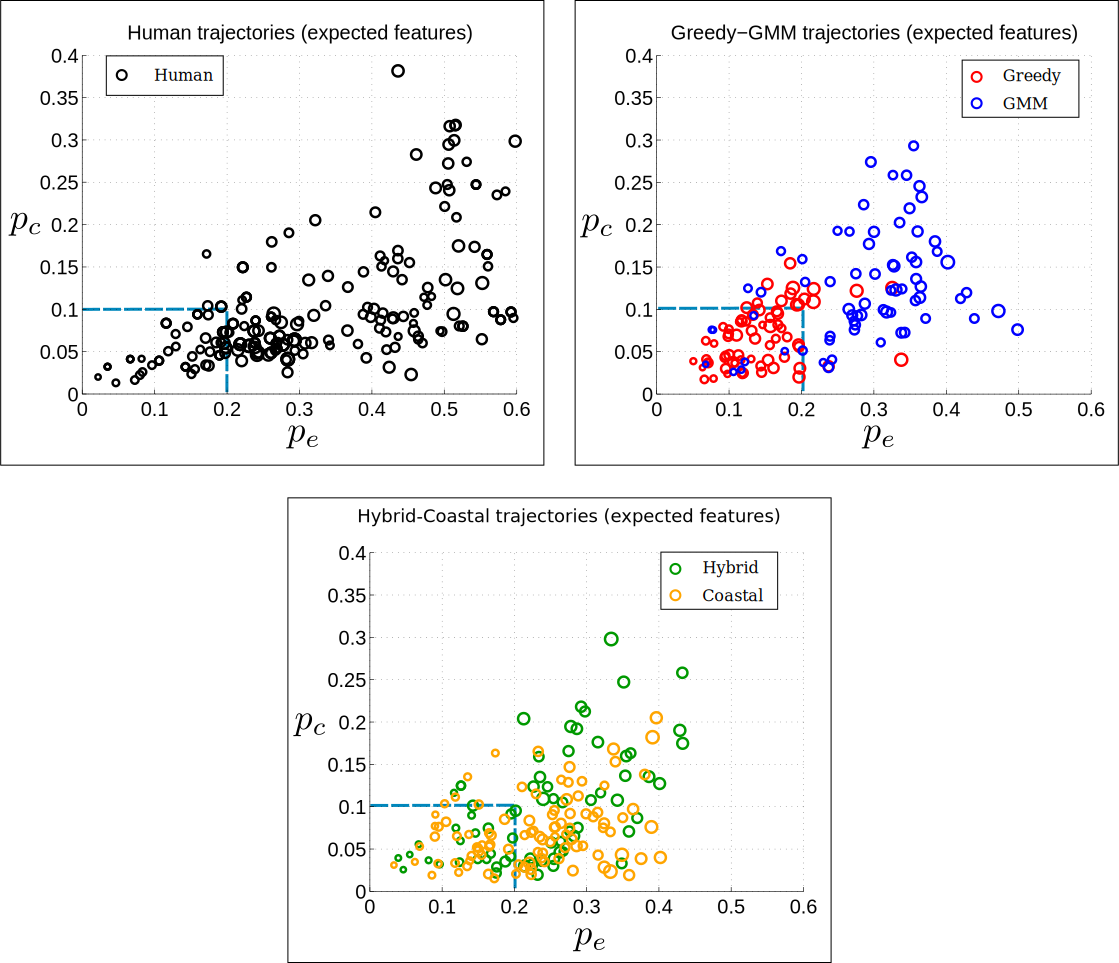
\includegraphics[width=\textwidth]{Figure6.pdf}
 \caption{Time evolution of both the joint and marginal distributions of the agent (blue) and object (red) probability distributions for 
 the case of a 1D search. The space is discretised to 100 bins and the agent is moving in the direction of the black arrow. 
 The black line represents the measurement likelihood function. It is along this line $A=O$ that the joint distribution will be
 changed. On the \textit{Left}, the measurement likelihood causes all the mass of joint distribution
 lying on the line $A=O$ to be removed. 
 The reason for this is that the agent has not sensed the object (the red and blue circles on the marginals indicate the true position of
 both the agent and the object), and all the probability mass which lies in the area of influence of the measurement likelihood gets 
 removed and redistributed to the other states in the joint distribution due to normalisation.}
 \label{fig:margina_joint_example}
\end{figure}

\paragraph{Parametrisation of MLMF-SLAM}

The parametrisation of the MLMF is also based on the standard SLAM graphical model Figure \ref{fig:bayesian_sse_dag}. However
we do not take a recursive approach but rather remember all measurement functions which have been applied since 
the state, see Equation \ref{eq:memory_function}-\ref{eq:joint_filter_memory}.

\begin{align} 
 P(A_{t-1},O|Y_{0:t-1},u_{0:t-1}) &= P(A_0) \cdot P(O)  \cdot  P(Y_0|A_0,O) \cdot \prod\limits_{t=1}^{t-1} P(A_t|A_{t-1},u_t) \cdot P(Y_t|A_t,O) \label{eq:memory_function} \\
 P(A_t,O|Y_{0:t},u_{0:t})         &= \frac{P(Y_t|A_t,O) \cdot  P(A_t,O|Y_{0:t-1},u_{0:t})  }{  P(Y_t|Y_{0:t-1}) } \label{eq:joint_filter_memory}
\end{align}

The filter is composed of the original marginal distributions $P(A_0)$ and $P(O)$ and a memory/history term $P(A_{t},O|Y_{0:t-1},u_{0:t})$. 
The memory function, Equation \ref{eq:memory_function}, consists of the set of measurement likelihood functions which have been applied 
since initialisation up to the current time step. The motion update consists of applying the forward dynamics $P(A_t|A_{t-1},u_t)$ to 
$P(A_{t-1},O|Y_{0:t-1},u_{0:t-1})$ (Equation \ref{eq:memory_function}) to achieve $P(A_t,O|Y_{0:t-1},u_{0:t})$, see Equation \ref{eq:time_update_memory}. 

\begin{align}\label{eq:time_update_memory}
 P(A_t,O|Y_{0:t-1},u_{0:t}) &= \sum\limits_{A_{t-1}} P(A_t|A_{t-1},u_t) \cdot  P(A_{t-1},O|Y_{0:t-1},u_{0:t-1})
 \end{align}

At every time step a new measurement likelihood function and dynamics is added to Equation \ref{eq:memory_function}.
The intuition of these two updates is as follows. At the first time step (after initialisation) we add the first measurement 
likelihood function which results in the line shown in Figure \ref{fig:margina_joint_example} \textit{left}. 
Then a motion update (agent moves towards state 100) is applied and this line (or measurement
likelihood function) shifts along the agent's axis by the displacement caused by the forward model and a new line is added at $A=O$, 
which is the result of the current measurement after the motion update. Repeating this process results in the white band present 
in Figure \ref{fig:margina_joint_example} \textit{right}. 

For ease of notation from this point onwards we will not show the conditioned actions $u_{0:t}$, so $P(A_t,O|Y_{0:t},u_{0:t})$ will 
be $P(A_t,O|Y_{0:t})$. 

\subsection{Computation of evidence and marginals}

In order to compute the marginal likelihood (also known as evidence) $P(Y_t|Y_{0:t-1})$ and the filtered  marginals $P(A_t|Y_{0:t})$,
$P(O|Y_{0:t})$ efficiently we take advantage of the fact that only a very small area 
in the joint distribution space will be affected by the measurement likelihood function at each time step.

Without lost of generality the measurement function will only make a difference to dependent $A \cap O$ regions in the joint distribution. 
The region inside the symmetric difference $A \ominus O$, will not be affected.
Figure \ref{fig:overlap_dependence_independence} shows the relation between the measurement 
function $P(Y_t|A_t,O)$ and the joint distribution $P(A_t,O)$ for three different initialisations. 

%\begin{FPfigure}
 \begin{figure}
 \centering
  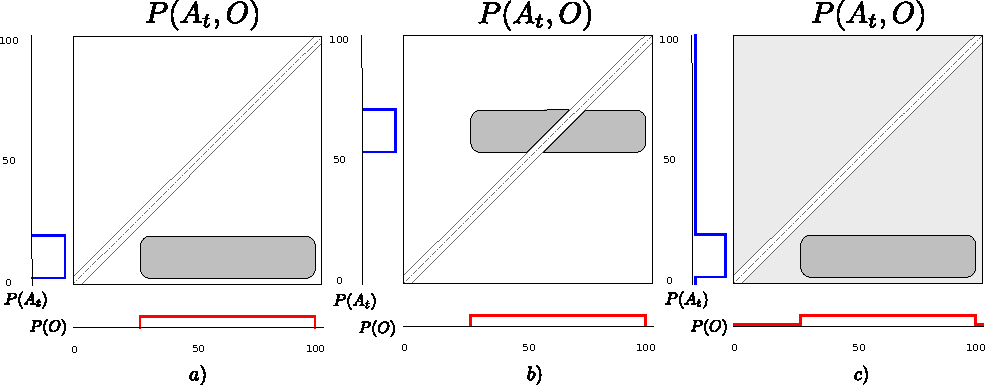
\includegraphics[width=\textwidth]{Figure7.pdf}
  \caption{
 $P(Y_t|A_t,O)$ effect on the joint distribution for three different initialisations. 
  The tube area depicts the regions where the measurement function influences the joint distribution. 
  The tube's boundary is governed by the bandwidth of the radial basis function of the measurement likelihood function.
  The joint distribution can be decomposed into a dependent $A \cap O$ (the intersection of $A$ and $O$) and independent $A \ominus O$ term 
  (the symmetric difference of $A$ and $O$, everything outside the area of intersection but still within the red and blue circles). 
  In the three other figures any probability mass of the joint  distribution which lies in the tube will be in the $\cap$, all probability 
  mass outside the tube but still within the grey rectangle is located in $\ominus$ and 
 the white space is in the domain but not parametrised and thus not considered. \textbf{a)} The initial configuration, the agent and object pdfs 
 are not overlapping and thus are completely independent. The joint distribution is not intersecting with the measurement function.
 \textbf{b)} The marginals overlap one another resulting in the measurement likelihood function intersection with the joint distribution.
 The probability mass at the intersection gets removed and renormalised to other regions which is the result of applying Bayes integration. 
 \textbf{c)} The marginals of $A$ and $B$ are completely overlapping, however only a small fraction of the probability mass in the joint distribution 
 is within the measurement function's tube.}
  \label{fig:overlap_dependence_independence}
\end{figure}
%\end{FPfigure}

As illustrated and explained in Figure \ref{fig:overlap_dependence_independence}, the joint distribution can be decomposed in a 
dependent and independent term (Equation \ref{eq:joint_independent_dependent}). 

\begin{equation}\label{eq:joint_independent_dependent}
 P(A_t,O|Y_{0:t}) = P_{\cap}(A_t,O|Y_{0:t}) + P_{\ominus}(A_t,O|Y_{0:t})
\end{equation}

The probability mass covered by the dependent term is located within the measurement function's tube and the independent probability mass 
is located outside as shown in Figure \ref{fig:overlap_dependence_independence}. This formulation will lead to large computational gain 
as the independent term is not influenced by the measurement function: $P_{\ominus}(A_t,O|\mathbf{Y_{0:t}}) \propto P_{\ominus}(A_t,O|\mathbf{Y_{0:t-1}})$.

\paragraph{Evidence}
The evidence of the measurement $P(Y_t|Y_{0:t-1})$ is the amount of probability mass which has be removed from the region of the joint 
distribution where the measurement likelihood function has had an impact. At time step $t$, the normalising factor to be added to 
the evidence is the difference between the probability mass located inside $A\cap O$ before the application of the measurement 
function $P(Y_t|A_t,O)$ and after (see Appendix \ref{appendix:evidence} for the full derivation).

\begin{align}
  P(Y_0) &= 1 - \overbrace{\sum\limits_{A_0}\sum\limits_{O} P_{\cap}(A_0,O|Y_0) - P(Y_0|A_0,O)\cdot P_{\cap}(A_0,O|Y_0)}^{\mathlarger{\mathlarger{\alpha_0}}}
\end{align}
The advantage of this form is that the summation is only over states which are in the dependent area $\cap$ of the joint 
distribution. This is generally always much smaller than the full space itself. By expanding the term $\alpha$ at time step $t$, 
we obtain a better intuition, see Equation \ref{eq:I}.
\begin{equation}\label{eq:I}
 \alpha_t =  \sum\limits_{A_t}\sum\limits_{O} P_{\cap}(A_t)\cdot P_{\cap}(O) \cdot P(Y_{0:t-1}|A_t,O)  - P(Y_t|A_t,O)\cdot P_{\cap}(A_t)\cdot P_{\cap}(O) \cdot P(Y_{0:t-1}|A_t,O) 
\end{equation}
The point of interest is that as we perform the filtering process we will never renormalise the whole joint distribution, but only keep 
track of how much it should have been normalised. To this end the original marginals $P(A_0)$ and $P(O)$  are never renormalised but are used 
to compute at each step how much of the probability mass $\alpha_t$ should go to the normalisation factor 
$P(Y_t|Y_{0:t-1}) = 1 - (\alpha_{0} + \alpha_{1} + \cdots + \alpha_{t})$. The evidence in question will never be negative, as the 
joint distribution sums to one and each $\alpha_t$ represents some of the mass removed from the joint distribution. Since we 
keep track of the history of applied  measurement likelihood functions we never remove the same amount of probability mass twice
from the joint distribution.


\paragraph{Marginals}

The computation of the marginal is similar to that of the evidence (see Appendix \ref{appendix:marginal} for the full derivation). 
The difference is that we do not marginalise the random variable being queried, so there is one less summation. 
As in the case for the evidence, the marginal is evaluated only in areas of the joint distribution which are dependent 
and it uses the previously computed evidence to normalise this region of the joint distribution during the marginalisation 
process.

\begin{equation}
 P(A_t,|Y_{0:t})  =  P(A_t|Y_{0:t-1}) - \Big(P_{\cap}(A_t|Y_{0:t-1}) -  P_{\cap}(A_t|Y_{0:t})  \Big) \label{eq:marignal_mrf} 
\end{equation}
\begin{equation}\label{eq:marignal_mrf_2}
 P_{\cap}(A_t|Y_{0:t}) = \sum\limits_{O} \frac{\overbrace{P(Y_t|A_t,O) \cdot P_{\cap}(A_t)\cdot P_{\cap}(O) \cdot P(Y_{0:t-1}|A_t,O)}^{P_{\cap}(A_t,O,Y_t|Y_{0:t-1})}}{\underbrace{1  - (\alpha_{0} + \alpha_{1} + \cdots + \alpha_{t-1})}_{P(Y_t|Y_{0:t-1})}}
\end{equation}

Note that it is a recursive process, $P(A_t,|Y_{0:\mathbf{t}})$ is computed in terms of  $P(A_t,|Y_{0:\mathbf{t-1}})$.

\subsection{MLMF-SLAM Algorithm}

\begin{algorithm}
\caption{MLMF-SLAM}
\textit{input}: $P^{*}(A_0), P^{*}(O), P(Y_0|A_0,O), \alpha=0$
 \begin{algorithmic}[1]
   \State{$P(A) = P^{*}(A)$} \Comment{initialise marginals (first time step)}
   \State{$P(O)   = P^{*}(O)$}
   \Statex{\textbf{Measurement Update}}
   \State{$P(A_t|Y_t) = P(A_t|Y_{0:t-1}) - \Big(P_{\cap}(A_t|Y_{0:t-1}) -  P_{\cap}(A_t|Y_{0:t}) \Big)$} 
   \State{$P(O|Y_t) = P(O|Y_{0:t-1}) -  \Big(  P_{\cap}(O_t|Y_{0:t-1}) -  P_{\cap}(O_t|Y_{0:t})\Big)$}
   \State{$\alpha = \alpha + \sum\limits_{A_t}\sum\limits_{O} P^{*}_{\cap}(A_t)\cdot P^{*}_{\cap}(O) - P(Y_0|A_t,O) \cdot P^{*}_{\cap}(A_t)\cdot P^{*}_{\cap}(O)$} \Comment{update normalisation factor}
   \State{$P(Y_{0:t-1}|A_t,O) \leftarrow P(Y_t|A_t,O) $} \Comment{update memory}
   \Statex{\textbf{Motion Update}}
   \State{$P(A_t|Y_t)  = \sum\limits_{A_{t-1}} P(A_t|A_{t-1},u_t) \cdot P(A_t|Y_t) $}
   \State{$P^{*}(A_t)  = \sum\limits_{A_{t-1}} P(A_t|A_{t-1},u_t) \cdot P^{*}(A_t) $}
   \State{$  P(A_t,O|Y_{0:t-1},u_{0:t}) = \sum\limits_{A_{t-1}} P(A_t|A_{t-1},u_t) \cdot  P(A_{t-1},O|Y_{0:t-1},u_{0:t-1}) $} 
\end{algorithmic} \label{alg:mrf-slam}
\textit{output:} $P(A_t|Y_{0:t-1})$, $P(O_t|Y_{0:t-1})$ 
\end{algorithm}

In Algorithm \ref{alg:mrf-slam} we give the motion-measurement update recursion for the MLMF-SLAM. The input parameters consist 
of all the marginals, the empty memory, the first measurement function and the amount of probability mass which has to be renormalised, $\alpha$. 
Note that the marginals with the superscript $(*)$ are the original marginals at initialisation. 
This formulation is advantageous as only the joint distribution is evaluated explicitly inside the tube 
$A\cap O$ created in the joint space by the measurement function. Through the term $P(Y_{0:t}|A_t,O)$ we keep track of the normalisation factor $P(Y_t|Y_{0:t-1})$ which 
is a scalar, and where we have previously applied the measurement function. 

We evaluated this formulation of the joint distribution with the standard histogram filter in the case of the 1D search routine 
illustrated in Figure \ref{fig:margina_joint_example} and we found them to be identical. We stayed true to the formulation of Bayes rule 
and thus assert that Algorithm \ref{alg:mrf-slam} is a Bayesian Optimal Filter/Solution
\footnote{An optimal Bayesian solution is an exact solution to the recursive problem of calculating the exact posterior density 
\cite{PF_tutorial_2002}}.

\section{Space \& time complexity (MLMF)}

For discussion purposes we consider the case of three beliefs, namely that of the agent and two other objects $O^{(1)}$ and $O^{(2)}$ but 
subsequently we generalise. As stated previously $M$ stands for the number of filtered random variables including the agent. When we refer 
to only the objects we say that we have $M-1$ random variables. $N$ is the number of discrete states in the world. We contrast
the MLMF with the histogram filter.

\subsection{Space complexity}

\paragraph{Histogram}

Figure \ref{fig:3bel_lik_profile} \textit{left} illustrates the volume occupied by the joint distribution for a marginal space of a 
100 states. The joint distribution $P(A,O^{(1)},O^{(2)})$ has $N^{M}$ parameters. 

\paragraph{MLMF}

Each random variable $X$ requires two marginals $P^{*}(X)$ and $P(X)$ (see Algorithm \ref{alg:mrf-slam}). Given
$M$ random variables, the initial number of parameters is $M \cdot (2 \cdot N)$. At every time step we store 
the action, $u_t \in D$, only if the current marginals have changed as a result of the measurement likelihood function, $P(Y_t|A_t,O)$.
Given a state space of size $N$, there can be no more than $N$ different measurement functions (one for each state). In
the worst case scenario the space complexity of the memory will be $D\cdot N$. The final worst case space complexity is
$M \cdot (2 \cdot N) + D \cdot N$. In 1D all measurement functions will form a closed convex set so we only need to 
keep track of the boundaries (two of them) giving a space complexity of  $M \cdot (2 \cdot N) + 2$.


\begin{figure}
 \centering
  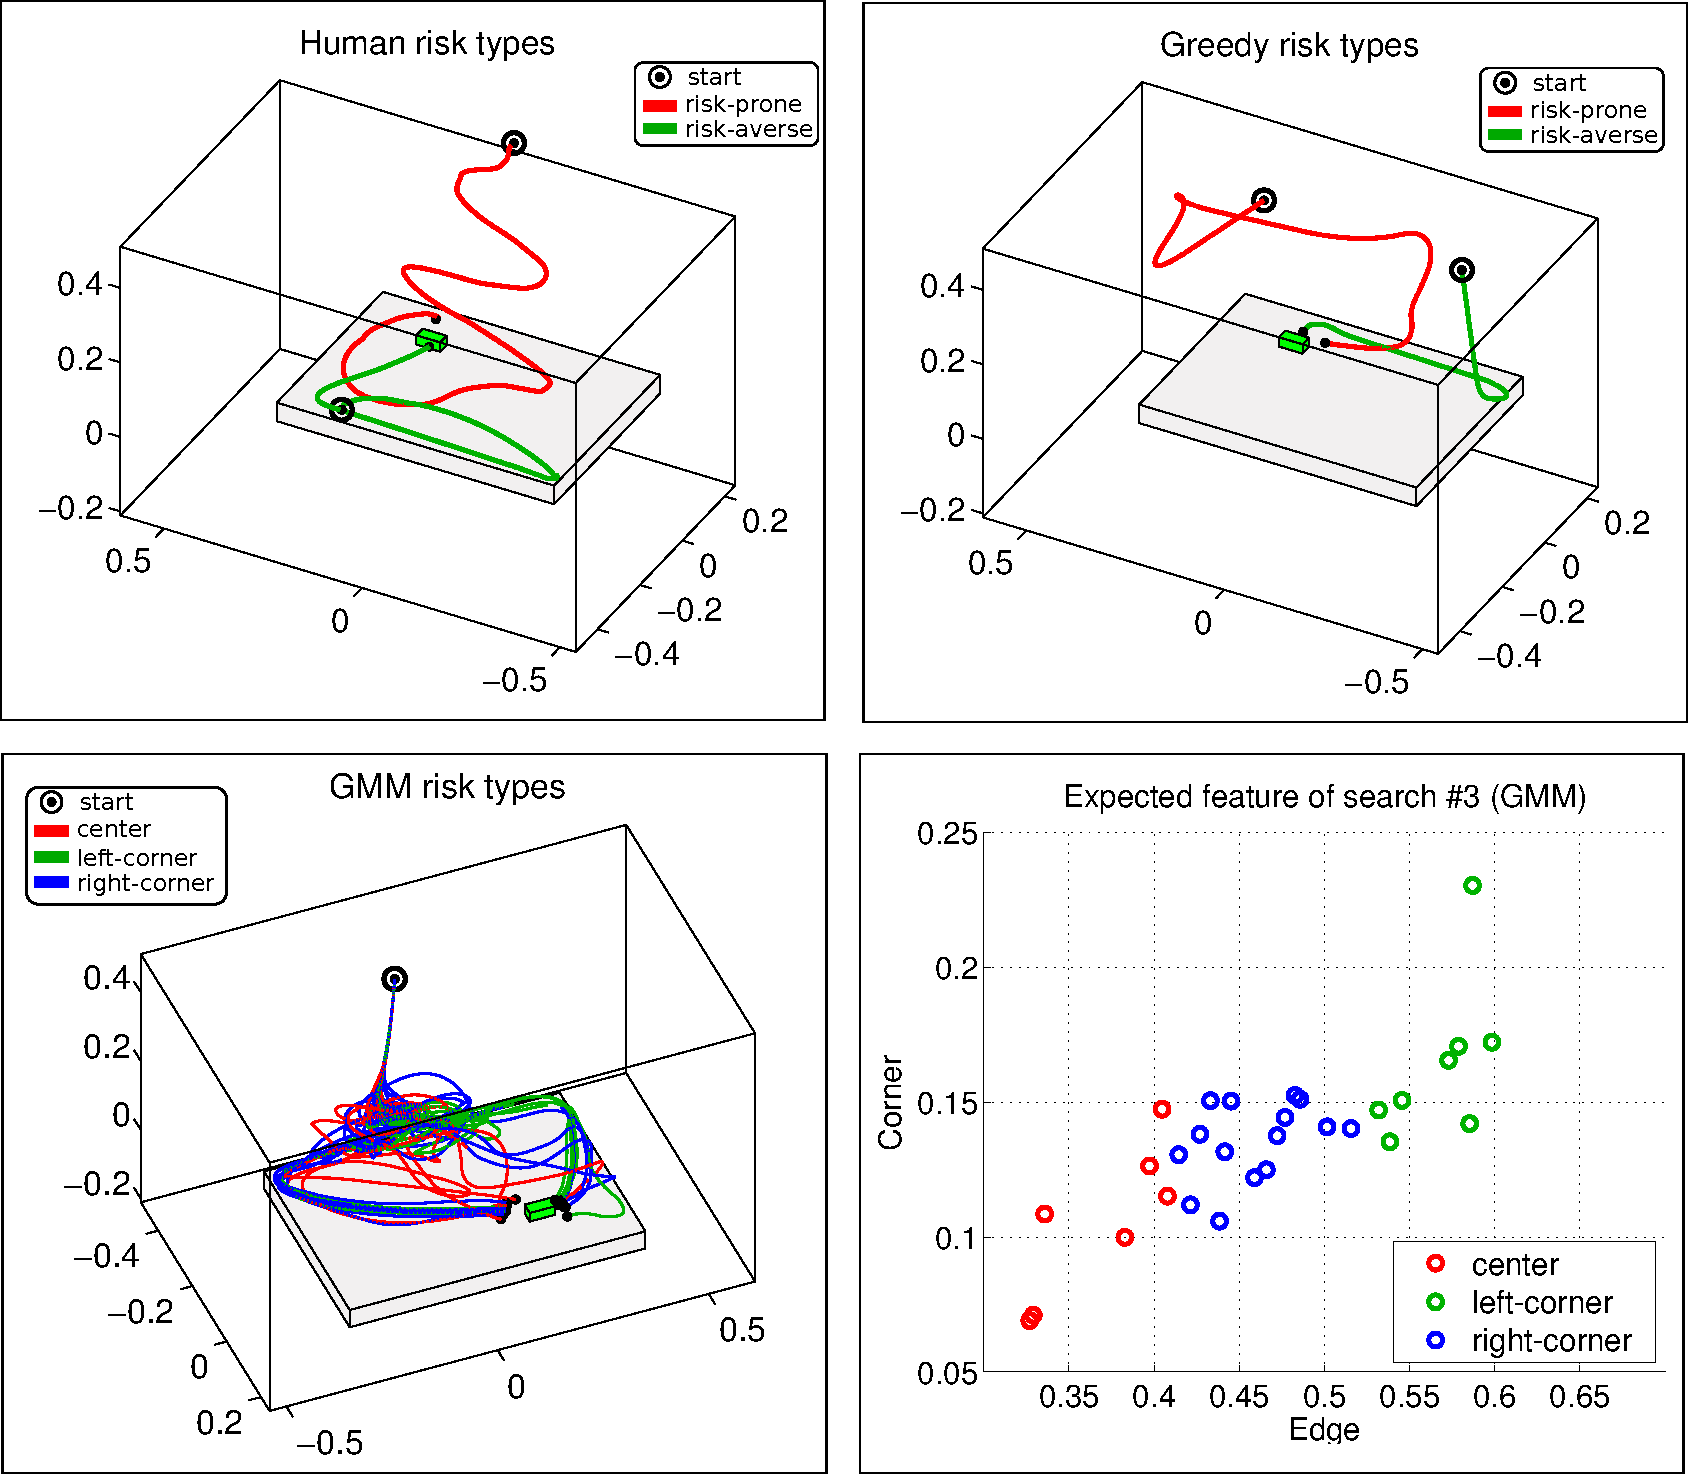
\includegraphics[width=0.9\textwidth]{Figure8.pdf}
  \caption{\textit{left:} Joint distribution $P(A,O^{(1)},O^{(2)})$ of the agent and two objects. Each measurement likelihood function, $P(Y|A,O^{(1)})$, 
  $P(Y|A,O^{(2)})$ and $P(Y|O^{(1)},O^{(2)})$ corresponds to a hyperplane in the joint distribution. The measurement function $P(Y|O^{(1)},O^{(2)})$ 
  stipulates that the objects cannot be in the same state. The marginal space is discretised to $N = 100$ states giving the total number of states in 
  the joint distribution as $100^3$ $(M=3)$. \textit{right:} Joint distribution of the agent and one object $P(A_t,O|Y_{0:t})$. Three measurement 
  functions have been added to the memory term. At every time step when an action is taken all measurement functions are updated according to 
  the action applied $u_t$. This means that the first function to be added to the memory will have had all actions applied to it. The number 
  of the equations and their associated lines in the plot indicate the order in which they have been added to the memory. 
  The three points are candidates at which we want to evaluate the joint distribution. First the offset $A=O+c$
  is evaluated which corresponds to the dotted red lines. Then these are checked against all the offsets stored in memory. The cost of evaluating
  the joint distribution at the yellow point is $\BigO{1}$ since we only have to check the first element in the memory. For the green and cyan points the 
  cost is $\BigO{\log(n)}$, where $n$ is the current size of the memory.}
  \label{fig:3bel_lik_profile}
\end{figure}

\subsection{Time complexity}

\paragraph{Histogram}
The computational cost of the histogram filter is equivalent to that of the space complexity, $\BigO{ N^M }$.

\paragraph{MLMF}

Every state in the joint distribution's state space which has been changed by the measurement likelihood function has to be
evaluated in Algorithm \ref{alg:mrf-slam}. As a result the computational complexity is directly related to the number 
of affected states. In Figure \ref{fig:3bel_lik_profile} \textit{left}, the number of effected states are those in the blue
and red plane (the states in the green plane will only be changed once because the agent's motion is parallel to it).
For $M$ random variables the computational cost is $\BigO{(M-1) \cdot N^{M-1}}$ as opposed to $\BigO{ N^M }$. The computation complexity
in this setup is still exponential but to the order $M-1$ as opposed to $M$ which will nevertheless quickly limit the scalability as more objects are added. 

\paragraph{Evaluation of a state in the joint distribution}

In Figure \ref{fig:3bel_lik_profile} (right) we show three different points in the joint distribution to be evaluated. The memory of applied measurement functions 
is searched to see if any have effected the values at the three chosen the states. The memory functions are sorted according to their offset from the axis $A=O$. For the yellow point the
cost is of $\BigO{1}$ since we only have to check the first (last) element in the list. For the green and blue point
the search is $\BigO{\log(n)}$, where $n$ is the number of stored memory functions (there can be no more than $N$, the total number of states). 


\section{Scalable extension to multiple objects}\label{subsec:scalabe_extension}

To make our filter scalable we introduce an independence assumption between the objects and model the joint distribution (Equation \ref{eq:pair_wise_joint}) as the product 
of agent-object pairs

\begin{equation}\label{eq:pair_wise_joint}
 P(A_t,O^{(1)},\cdots,O^{(M-1)}|Y_{0:t}) = \prod\limits_{i=1}^{M-1} P(A^{(i)}_t,O^{(i)}|Y^{(i)}_{0:t})
\end{equation}

The measurement variable $Y_t$, is the vector of all each agent-object 
measurement pairs, $Y_t = \left[Y^{(1)}_t,\dots,Y^{(M-1)}_t\right]^{\mathrm{T}}$. Each agent-object joint distribution has its own parametrisation of the agent's marginal,
$A^{(1)}_t,\dots,A^{(M-1)}_t$ which combine to give the overall marginal of the agent $A_t$.

\begin{figure}
\centering
  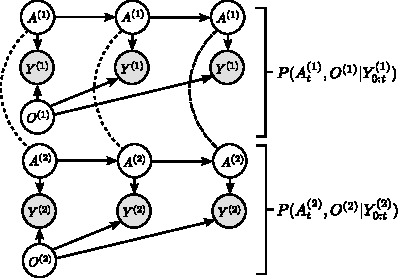
\includegraphics[width=0.5\textwidth]{Figure9.pdf}
  \caption{\textbf{Scalable filter} Each agent-object joint distribution pair is modelled independently. For clarity we have left 
  out the action random variable $u$ which is linked to every agent node.
  Two joint distributions $P(A^{(1)},O^{(1)}|Y^{(1)}_{0:t})$   and $P(A^{(2)},O^{(2)}|Y^{(2)}_{0:t})$ parametrise the graphical model. 
  The dashed undirected lines represent a wanted dependency, if present $O^{(1)}$ and $O^{(2)}$ are to be dependent through $A$. In
  the standard setting there will be no exchange of information between the individual joints. However we demonstrate later on how
  we perform a one time transfer of information when one of the objects is sensed.}
  \label{fig:scalable_mlmf_dae}
\end{figure}

The computation of each object marginal $P(O^{(i)}|Y^{(i)}_{0:t})$ is independent of the other objects. This is evident from the marginalisation 
see Equation \ref{eq:marg_indep}-\ref{eq:marg_indep_prod}.

\begin{align}
 P(O^{(i)}|Y^{(i)}_{0:t}) &= \sum\limits_{A^{(i)}_t} P(A^{(i)}_t,O^{(i)}|Y^{(i)}_{0:t}) \label{eq:marg_indep} \\
 P(A_t|Y_{0:t})   &= \prod\limits_{i=1}^{M-1} \left(\sum\limits_{O_i} P(A^{(i)}_t,O^{(i)}|Y^{(i)}_{0:t})\right)  \\
	    &= \prod\limits_{i=1}^{M-1} \ P(A^{(i)}_t|Y^{(i)}_{0:t}) \label{eq:marg_indep_prod}
\end{align}

The independence assumption will create an unwanted effect with respect to agent's marginal $P(A_t|Y_{0:t})$. 
At initialisation the agent marginals should all be equal, $P(A_0|Y_0) = P(A^{(i)}_0|Y^{(i)}_0) \forall_i$ however this is not the case because of 
Equation \ref{eq:marg_indep_prod}. To overcome this we define the final marginal, $P(A_t|Y_{0:t})$, of the agent as being the average of all the individual
pairs $P(A^{(i)}|Y^{(i)}_{0:t})$.

\begin{equation}
  P(A_t|Y_t) := \frac{1}{M-1} \sum\limits_{i=1}^{M-1} \ P(A^{(i)}_t|Y^{(i)}_t) \label{eq:marg_indep_sum}
\end{equation}

Figure \ref{fig:scalable_mlmf_dae}, depicts the graphical model of the scalable formulation. 
As each joint distribution pair has its own parametrisation of the agent's marginal and these do not subsequently get updated by one another,
the information gained by one joint distribution pair is not transferred.
A remedy is to transfer information between the marginals $A^{(i)}$ at specific intervals namely when one of the objects is sensed by the agent. 


\begin{algorithm}
\caption{Scalable-MLMF: Measurement Update}
\textit{input}: $\{P^{*}(A^{(i)}_t),P(A^{(i)}_t|Y^{(i)}_{0:t-1}),P^{*}(O^{(i)}),P(O^{(i)}|Y^{(i)}_{0:t-1}),Y^{(i)}_t\}^{i=1\cdots (M-1)}$
  \begin{algorithmic}[1]
  \If {$Y^{(i)}_t > 0$} \Comment{Object $i$ has been sensed by the agent}
      \State{$P(O^{(i)}|Y^{(i)}_{0:t}) \leftarrow P(O^{(i)}|Y^{(i)}_{0:t-1})$} \Comment{Measurement Update Algorithm \ref{alg:mrf-slam}}   
      \State{$P(A^{(i)}_t|Y^{(i)}_{0:t}) \leftarrow P(A^{(i)}_t|Y^{(i)}_{0:t-1})$} 
      \ForAll {$j\in(1,\dots M-1) \setminus i$} 
	\State{$P(A^{(j)}_t) = P(A^{(i)}_t)$}
	\State{$P^*(A^{(j)}_t) = P^*(A^{(i)}_t)$}
	\State{$P(O^{(j)}|Y^{(i)}_{0:t}) \leftarrow \sum\limits_{A^{(j)}} P(A^{(j)}_t,O^{(j)}|Y^{(i)}_{0:t})$} \Comment{re-compute object $(j)$ marginal}
      \EndFor 
\vspace{-1em}	\Else
      \State{Measurement Update Algorithm \ref{alg:mrf-slam}}
  \EndIf
\end{algorithmic} \label{alg:scalabe-mrf-slam}
\end{algorithm}


Figure \ref{fig:transfer_information}, depicts the process of information exchange between object $O^{(1)}$ and $O^{(2)}$ in the event that the agent 
gets a positive sensation of $O^{(2)}$. Prior to the positive detection both marginals $P(A^{(1)}_t|Y^{(1)}_{0:t-1})$ and $P(A^{(2)}_t|Y^{(2)}_{0:t-1})$ 
occupy the same region and are identical. When the agent senses $O^{(2)}$ the line defined by the measurement 
likelihood function $P(Y^{(2)}_t|A^{(2)}_t,O^{(2)})$ becomes a hard constraint implying that both the agent and $O^{(2)}$ have to satisfy this constraint.
The exchange of information of one joint distribution to another is achieved through the agent's marginals $A^{(i)}$ according to Algorithm \ref{alg:scalabe-mrf-slam}.
The measurement update is the same as previously described in Algorithm \ref{alg:mrf-slam} in the case of no positive measurements of the objects. If the agent
senses an object, all of the agent marginals of the remaining joint distributions are set to the marginal of the joint distribution pair belonging to the positive 
measurement $Y^{(i)}_t$. The result of applying the constraint by setting the agent's marginals equal is depicted in the \textit{bottom left} of Figure \ref{fig:transfer_information}.

\begin{figure}
  \centering
  \fbox{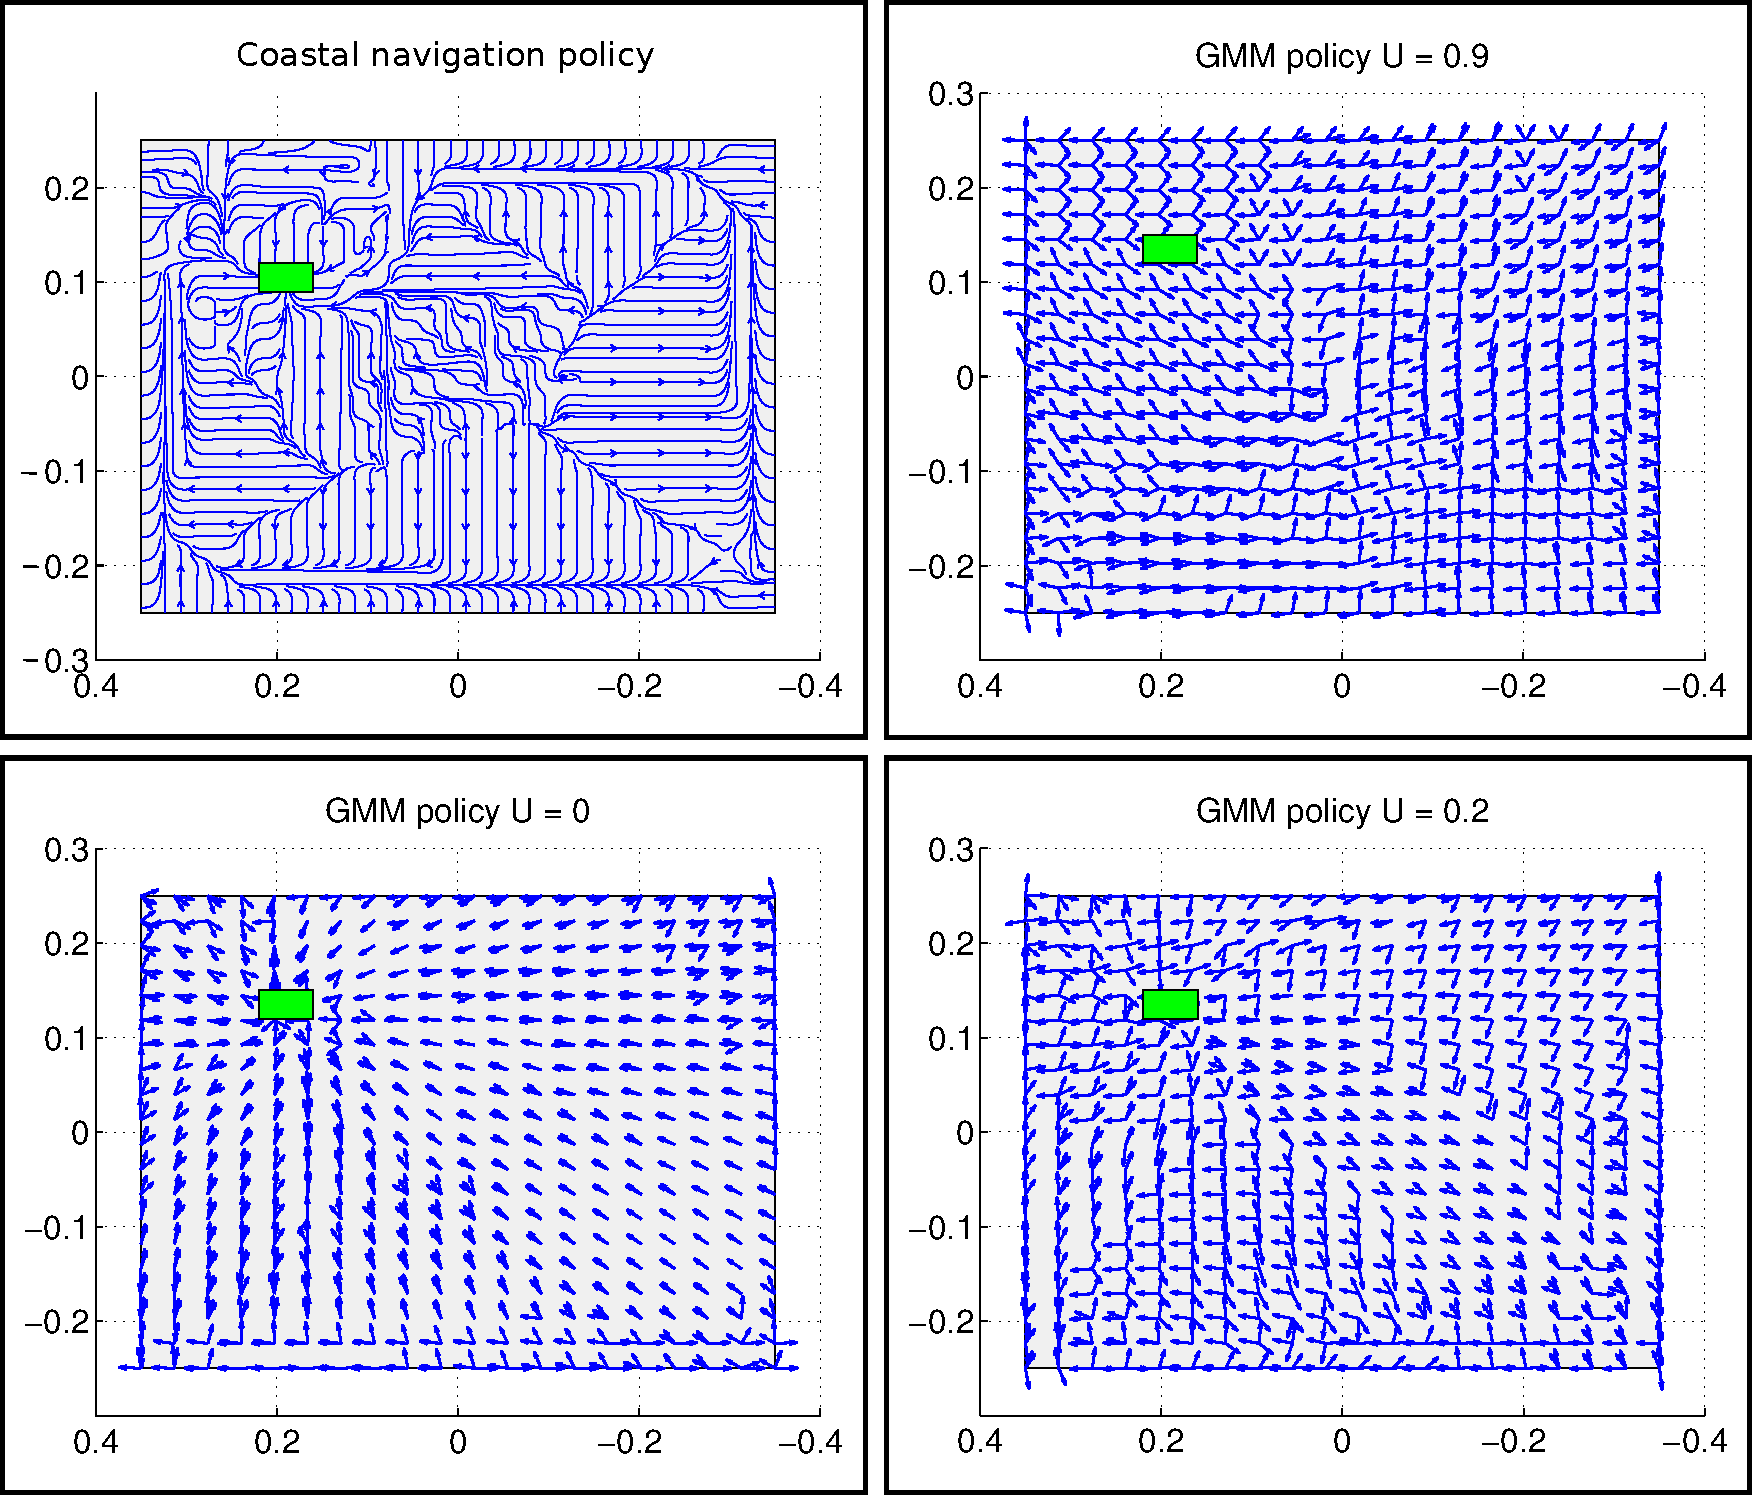
\includegraphics[width=0.8\textwidth]{Figure10.pdf}}
  \caption{\textbf{Transfer of information between joint distributions} \textit{top left and right:} Joint distributions of 
   $P(A^{(1)}_t,O^{(1)}|Y^{(1)})$ and $P(A^{(2)}_t,O^{(2)}|Y^{(2)})$ prior and post sensing. The red and blue lines correspond 
  to the region in which the measurement functions $P(Y^{(1)}_{t}|A^{(1)}_t,O^{(1)})$ and $P(Y^{(2)}_{t}|A^{(2)}_t,O^{(2)})$ will change the joint distributions.
  The dotted black lines are for ease of comparing the joint distributions prior and post sensing.
  \textit{bottom right:}  After the agent has sensed $O^{(2)}$, all the probability mass which was not overlapping the blue line becomes an infeasible
  solution to the agent and object locations. \textit{bottom left:} The constraint imposed by the measurement likelihood function of the second object
  (blue line) is transferred to the joint distribution of the first object according to Algorithm \ref{alg:scalabe-mrf-slam}.
  The result is a change in the joint distribution  $P(A^{(1)}_t,O^{(1)}|Y^{(1)})$, which satisfies the constraints 
  imposed by the agent's marginal from the joint distribution $P(A^{(2)}_t,O^{(2)}|Y^{(2)})$.}
  \label{fig:transfer_information}
\end{figure}

Figure \ref{fig:independence_object} shows marginals resulting from the joint distributions in Figure \ref{fig:transfer_information}. The marginals in
the \textit{left} plot are the result after updating the marginals $A^{(i)}$. The \textit{right} plot is the result for the case where the objects
remain independent. 

The result of introducing a dependency between the objects through the agent's marginals in the event of a sensing and treating them
independently gives the same solution as the histogram filter in this particular case. However as each individual marginal $A^{(i)}_t$ diverges 
from the others the filtered solution will diverge from the histogram's solution. We assume however that the objects are weakly dependent 
and sharing information during positive sensing events would be sufficient. In section \ref{subsec:eval_indep_assumptiom} we will 
evaluate the independence assumption with respect to the histogram filter.

\begin{figure}
  \centering
  \fbox{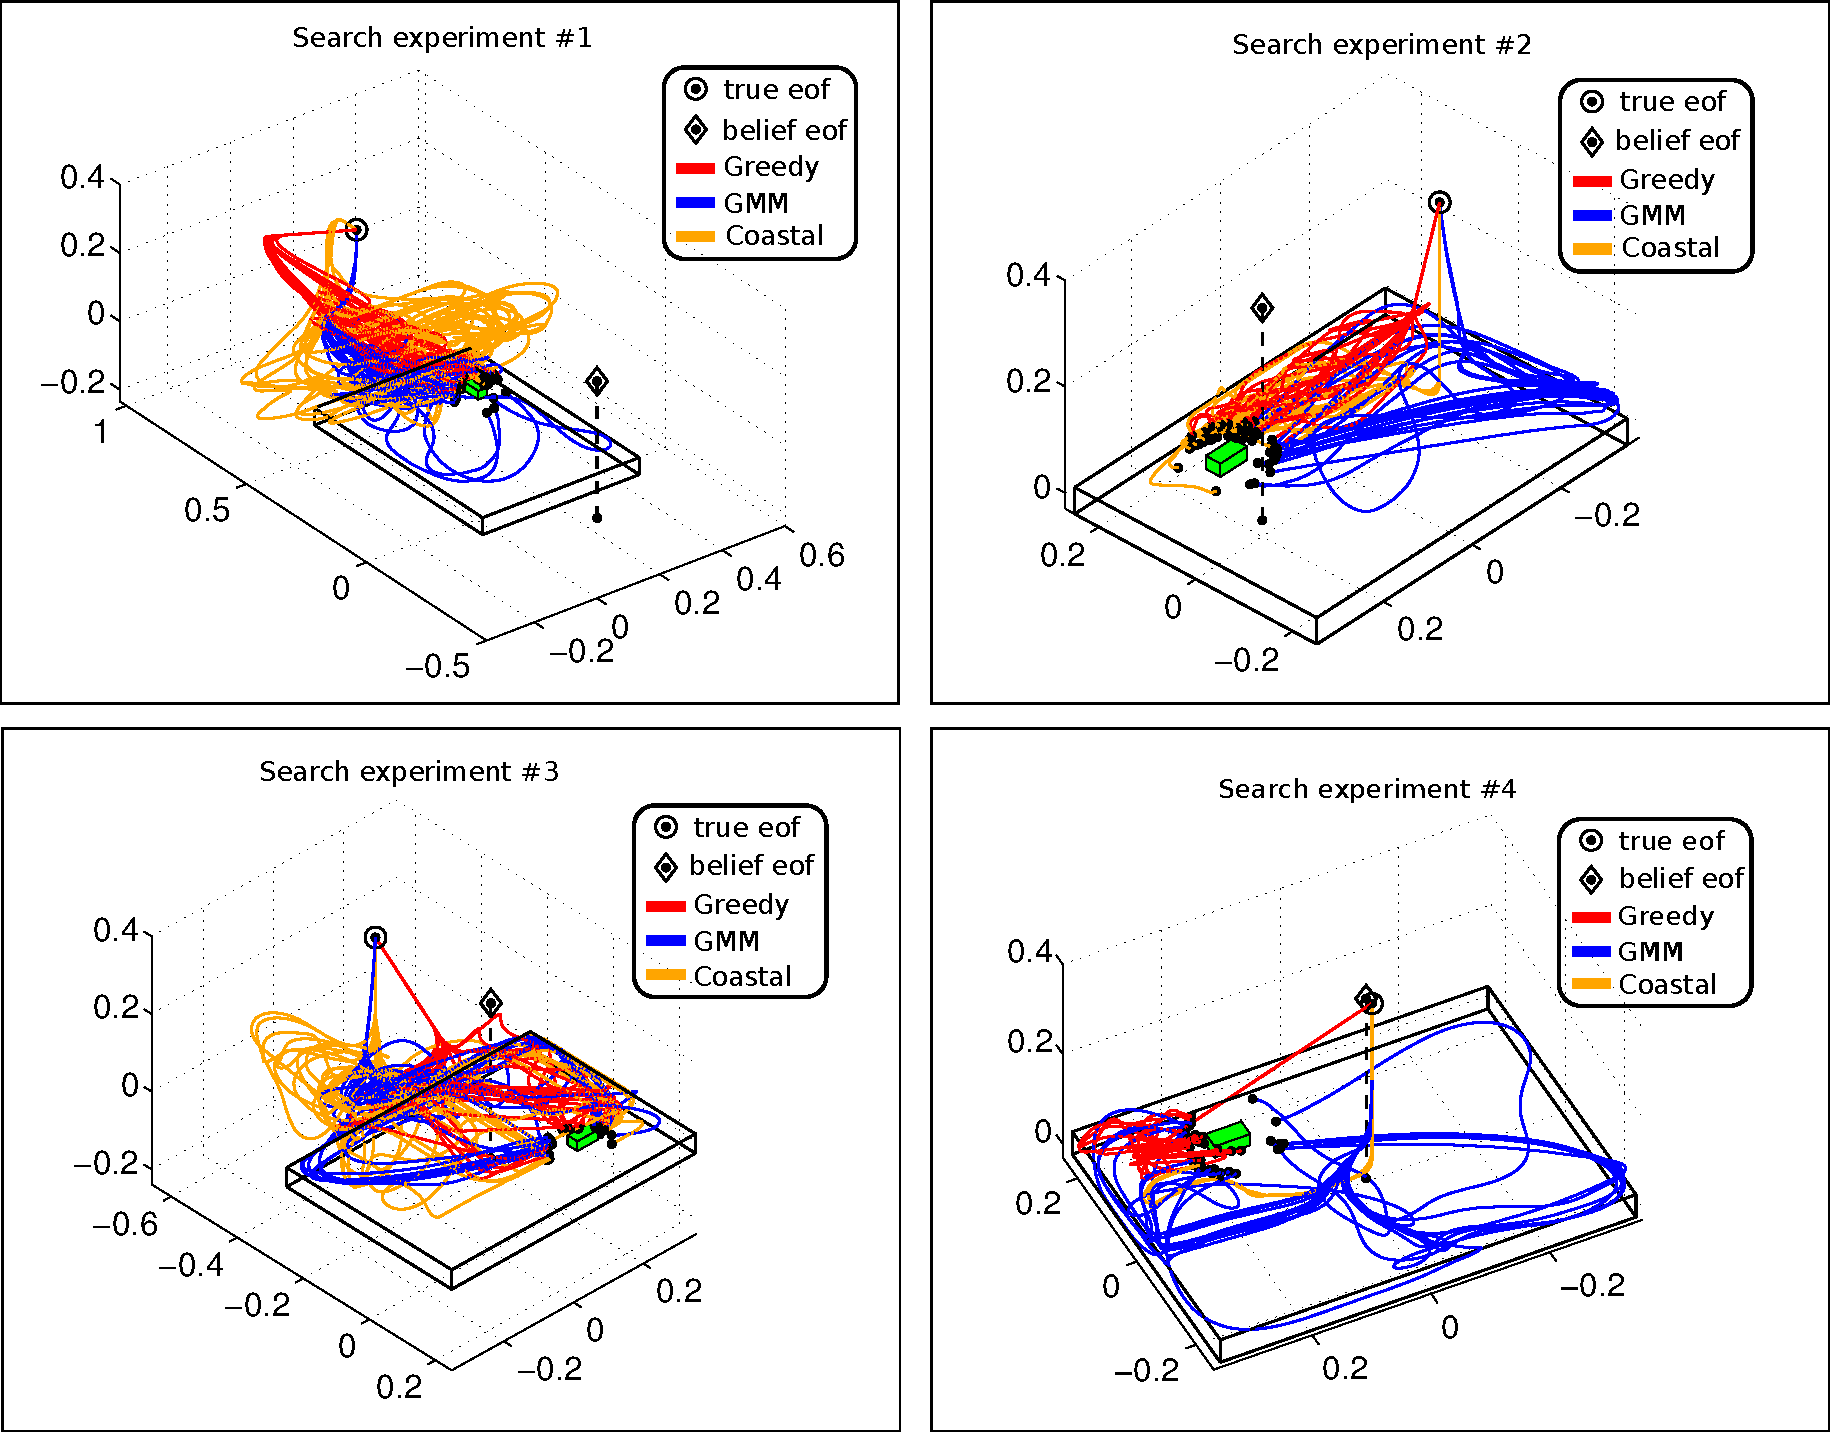
\includegraphics[width=0.8\textwidth]{Figure11.pdf}}
  \caption{\textbf{Independence \& Objects} \textit{left:} resulting marginals after setting the agent marginals of each pair wise joint distribution
  equal $A^{(1)}_t = A^{(2)}_t$ according to Algorithm \ref{alg:scalabe-mrf-slam}. The object marginal $P(O^{(2)}|Y_{0:t})$ is recomputed. 
  \textit{right:} resulting marginals in which the objects have no influence on one another. The difference
   between the two figures is that the object $O^{(1)}$ marginal changed in the case where we introduced the dependence \textit{left plot}, and remained 
  unchanged in the case where the objects are treated as being independent \textit{right plot}.}
  \label{fig:independence_object}
\end{figure}

Table \ref{tab:time_space_summary} summarises the time and space complexity for the three filters. In the case of transfer of
information between marginals the computational complexity is higher, however this is a one time occurrence. For the full derivation of
time and space complexity of the scalable-MLMF filter see Appendix \ref{appendix:space_time_scalable_mlmf}.

\begin{table}
 \centering
 \begin{tabular}{c|c|c|}
	         &    space   &     time \\ \hline
   histogram     &    $N^M$                                         &  $\BigO{N^M}$ \\ \hline
   MLMF          &    $M \cdot N \cdot \left(2 + D\right)$          &  $\BigO{(M-1) \cdot N^{(M-1)}}$ \\ \hline
   scalable-MLMF &    $(M - 1) \cdot N \cdot \left(4 + D\right)$    &  $\BigO{2 \cdot (M-1) \cdot N}$ \\ \hline
   \end{tabular}
   \caption{\textbf{Time and space complexity summary} For both MLMF and scalabe-MLMF the worst case scenario is reported for the space complexity.}
   \label{tab:time_space_summary}
\end{table}




\section{Evaluation}

We conduct three different types of evaluation to quantify the scalability and correctness of the scalable-MLMF filter. The first experiment
tests the scalability of our filter in terms of processing time taken per motion-measurement update cycle. The second experiment evaluates the independence 
assumption between the objects which was made in the scalable-MLMF filter. The third and final experiment determines the effect the memory size has 
on a search policy whose goal is to locate all the objects in the \textit{Table Top} world.

\subsection{Evaluation of time complexity}

We measured the time taken by the motion-measurement update loop, as a function of the number beliefs and number of states per belief. 
We started with a 100 states per belief and gradually increase it to 10'000'000 over 50 steps. For each of the 50 steps we went from 2 objects to 25. Figure \ref{fig:time_complexity} \textit{left} illustrates the computational
cost as a function of number of states and objects. For each state-object pair 100 motion-measurement updates were performed. Most of the trials returned time updates 
below 1 Hz. Figure \ref{fig:time_complexity} \textit{right} shows the computational cost as a function of the number of states plotted for 6 different filter runs with
a different number of objects. As the number of states increases exponentially so does the computational cost. Note the cost increases at the same
rate as the number of states meaning that the computational complexity is linear with respect to the number of states. This result is in agreement with 
the asymptotic time complexity.

\begin{figure}
 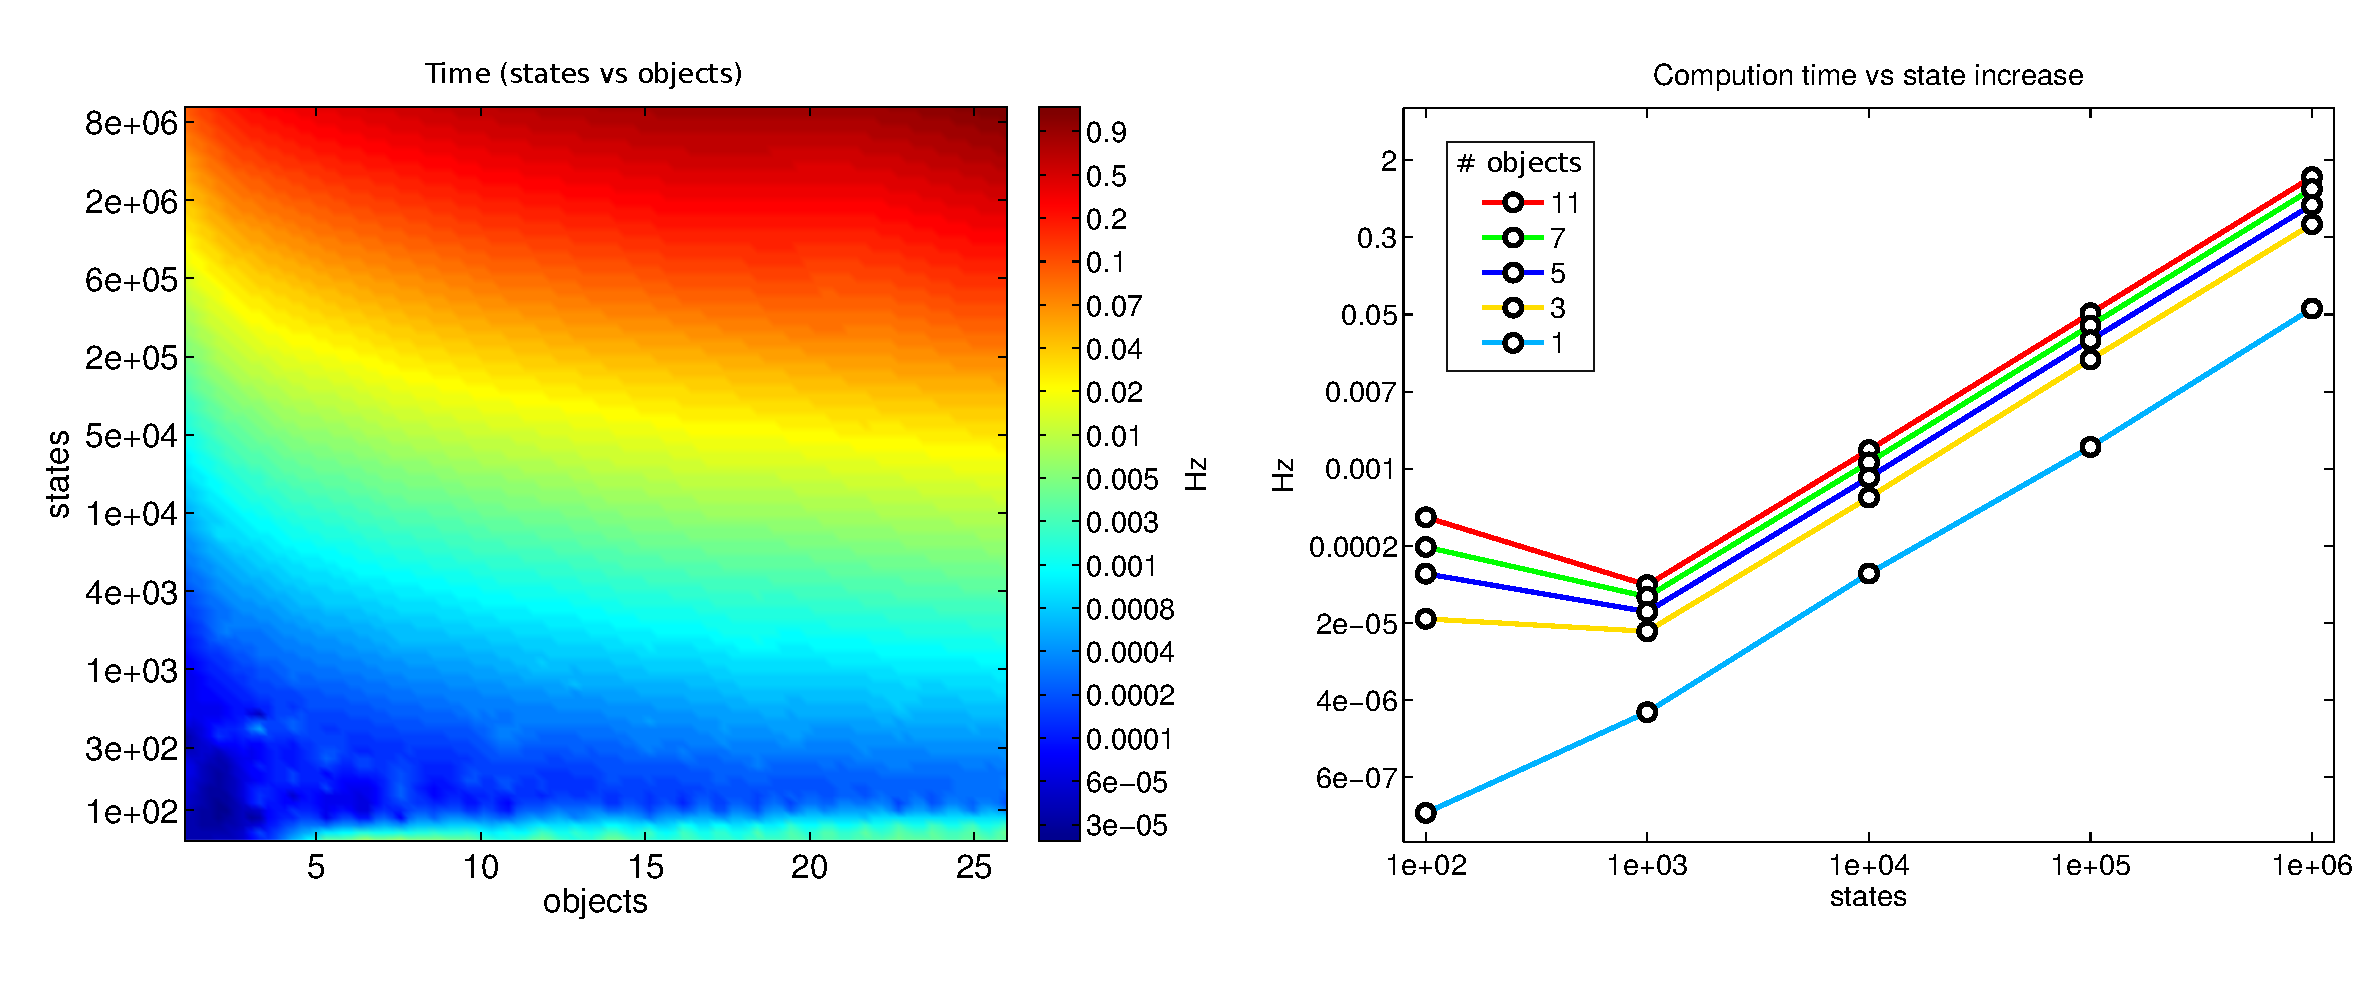
\includegraphics[width=\textwidth]{Figure12.pdf}
 \caption{\textbf{Time complexity:} \textit{left:} mean time taken in Hz for a loop update (motion and measurement) as a function of the number of states in a marginal and the 
 number of objects present. \textit{right:} time taken for a loop update with respect to the number of states in the marginal. The colour coded lines are 
 associated with the number of objects present. The computational cost is plotted on a log scale. As the number of states increases exponentially the
 computational cost matches it.}
 \label{fig:time_complexity}
\end{figure}


\subsection{Evaluation of independence assumption}\label{subsec:eval_indep_assumptiom}

In section \ref{subsec:scalabe_extension} we made the assumption (for scalability reasons) that the objects' beliefs are independent
from one another. To evaluate this assumption we compared our filter on three random variables, an agent and two objects with respect to the ground truth
which we obtain from the standard histogram filter. For each of the three beliefs (the agent and two objects), 100 different marginals 
were generated and the true locations (actual position of the agent and objects) were sampled from them. 
The agent carries out  a sweep of the state space for each of the 100 initialisations and the actual policy is saved 
and run with the scaled-MLMF filter. In the first experiment we assume that the objects are completely independent 
and that there is no transfer of information between the pair-wise joint distributions. In the second and third experiments we perform the exchange of information as 
described in Algorithm \ref{alg:scalabe-mrf-slam}. Here we compare the effect of using the product of the agent's marginals $P(A_t|Y_{0:t}) = P(A^{(1)}_t|Y^{(1)}_{0:t}) \cdot P(A^{(2)}_t|Y^{(2)}_{0:t})$ 
against their average $P(A_t|Y_{0:t}) = \frac{1}{2}P(A^{(1)}_t|Y^{(1)}_{0:t}) + \frac{1}{2}P(A^{(2)}_t|Y^{(2)}_{0:t})$. 

For each of the 100 sweeps we compared the ground truth given by the histogram filter and scalabe-MLMF using the Hellinger distance (Equation \ref{eq:hellinger}).
\begin{equation} \label{eq:hellinger}
 H(P,Q) = \frac{1}{\sqrt{2}}\, \|\sqrt{P} - \sqrt{Q}\|_2  
\end{equation}
The Hellinger distance is a metric which measures the distance between two probability distributions. Its value lies strictly between 0 (the two 
distributions are identical) and 1 (no overlap between them). Figure \ref{fig:independence_assumption_test} shows the kernel density 
distribution of the Hellinger distances taken at each time step for all 100 sweeps.

The best results were for case 3). The \textit{bottom plots} show that the Hellinger distance distribution between the
object marginals for both case 2) and 3) are the same. However there is a significant improvement when using the average of the agent's marginals as oppose to 
their product. 

\begin{figure}
 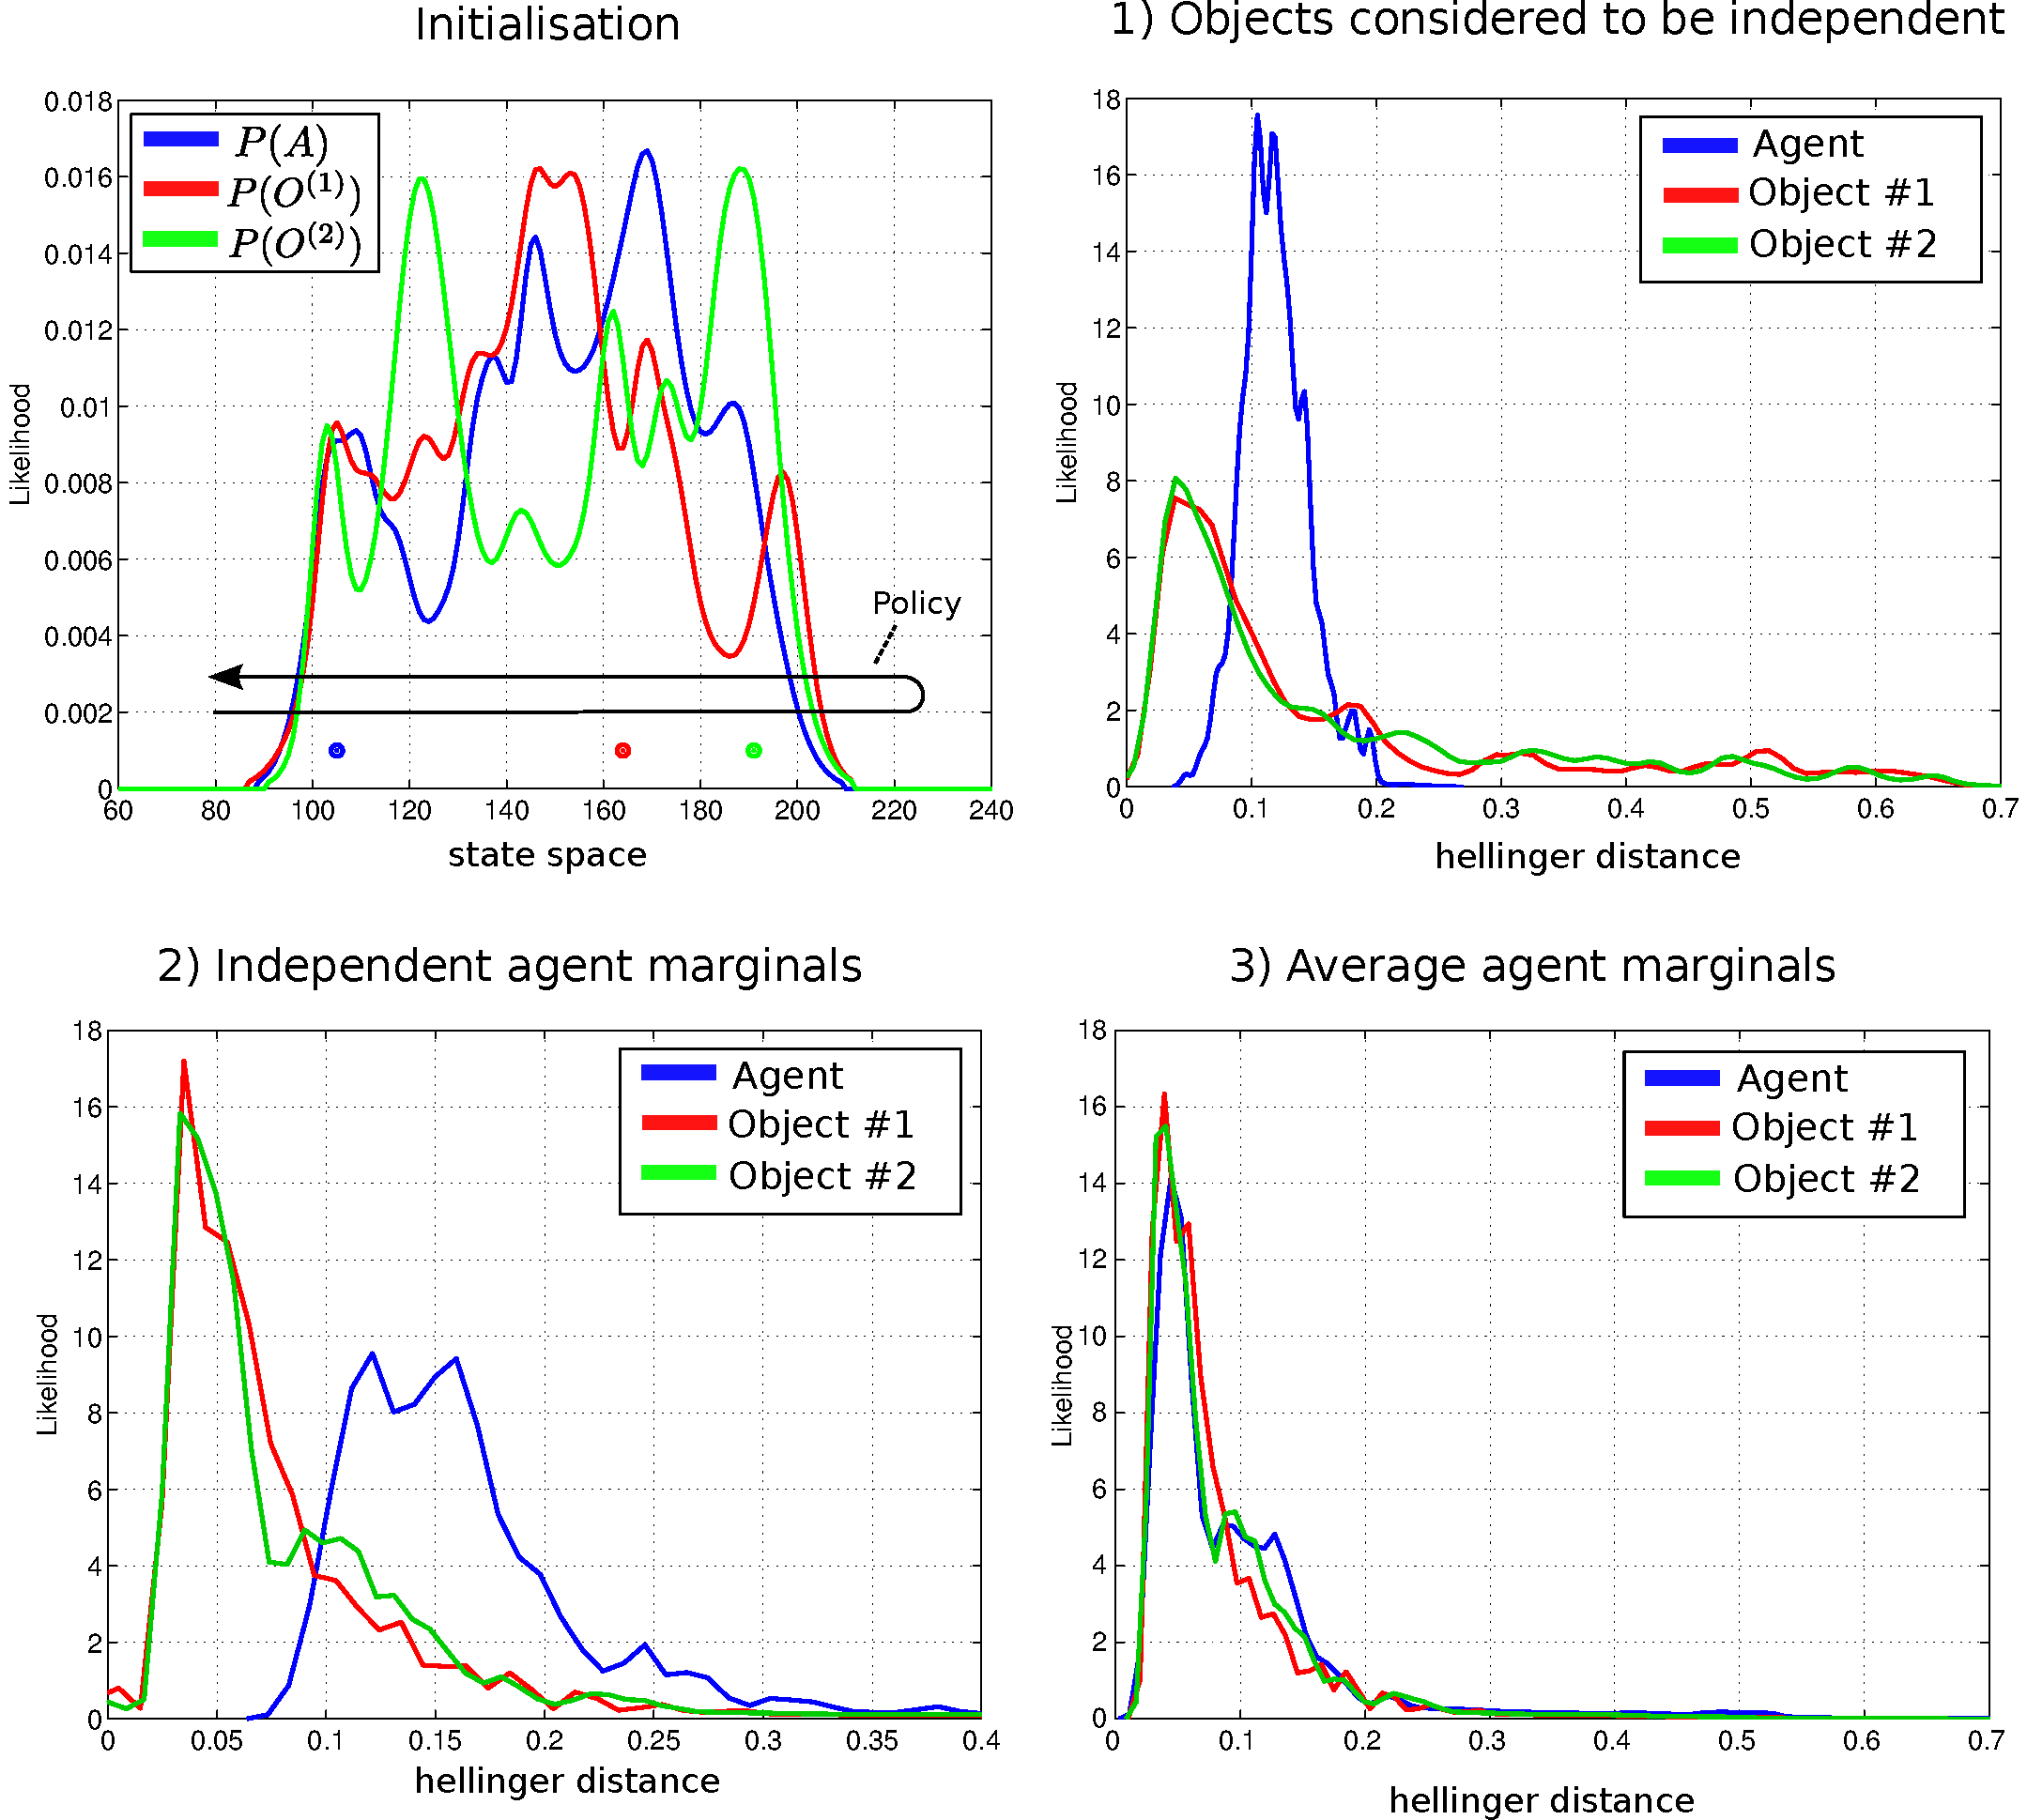
\includegraphics[width=\textwidth]{Figure13.pdf}
 \caption{\textbf{Comparison of scalable-MLMF and the histogram filter} A deterministic sweep policy was carried out for 100 different initialisations of 
 the agent and object beliefs. \textit{top left:} One particular Initialisation of the agent and object
 random variables. The true position of the agent and objects were sampled at random. The black arrow indicates the general policy which was 
 followed for each of the 100 sweeps. 
 These were performed for 1) scalable-MLMF  with objects considered to be independent at all times (no Algorithm \ref{alg:scalabe-mrf-slam}). 2) 
 Agent marginal $P(A_t|Y_{0:t})$ is the product of marginals $P(A^{(i)}_t|Y^{(i)}_{0:t})$ (Equation \ref{eq:marg_indep_prod}). 
 3) marginal $P(A_t|Y_t)$ is taken to be the average 
 of all marginals $P(A^{(i)}_t|Y^{(i)}_{0:t})$ (Equation \ref{eq:marg_indep_sum}).  For each of these three experiment we report the 
 kernel density estimation over the Hellinger distances taken at every time step between ground truth (from histogram filter) and scalable-MLMF.}
 \label{fig:independence_assumption_test}
\end{figure}

\subsection{Evaluation of memory}

The memory is the list of all measurement likelihood functions which have been applied on the joint 
distribution since initialisation. As detailed previously there can be no more than $N$ different measurement likelihood functions added to 
memory. In the case of a very large state space this might be cumbersome. We investigate how restricting the memory size 
can impact on the decision process in an Active-SLAM setting. Given our set up we choose a breadth-first search in the action 
space with a one time step horizon, making it a greedy algorithm. The objective function we utilise is the information
gain of the beliefs after applying an action (Equation \ref{eq:greedy_algorithm}).

\begin{equation}\label{eq:greedy_algorithm}
 u_{t} = \operatorname*{arg\,max}_{u_t} H\{P(A_{t-1},O|Y_{0:t-1},u_{0:t-1})\} - \mathbb{E}_{Y_t}\left[H\{P(A_{t},O|Y_{0:t},u_{0:t})\}\right]
\end{equation}

For each action we run the filter forward in time and sample from the measurement model since we cannot know ahead of time the actual 
measurement and have to estimate it. The information gain is the difference between the current entropy (defined 
by $H\{\cdot\}$) and the future entropy after the simulated motion and measurement update. The action with the highest information gain 
is subsequently selected. This is repeated at each time step. In Figure \ref{fig:exploration_init} we illustrate the environment setup for 
a 1D and 2D case. The agent's task is to find the objects in the environment.


\begin{figure}
  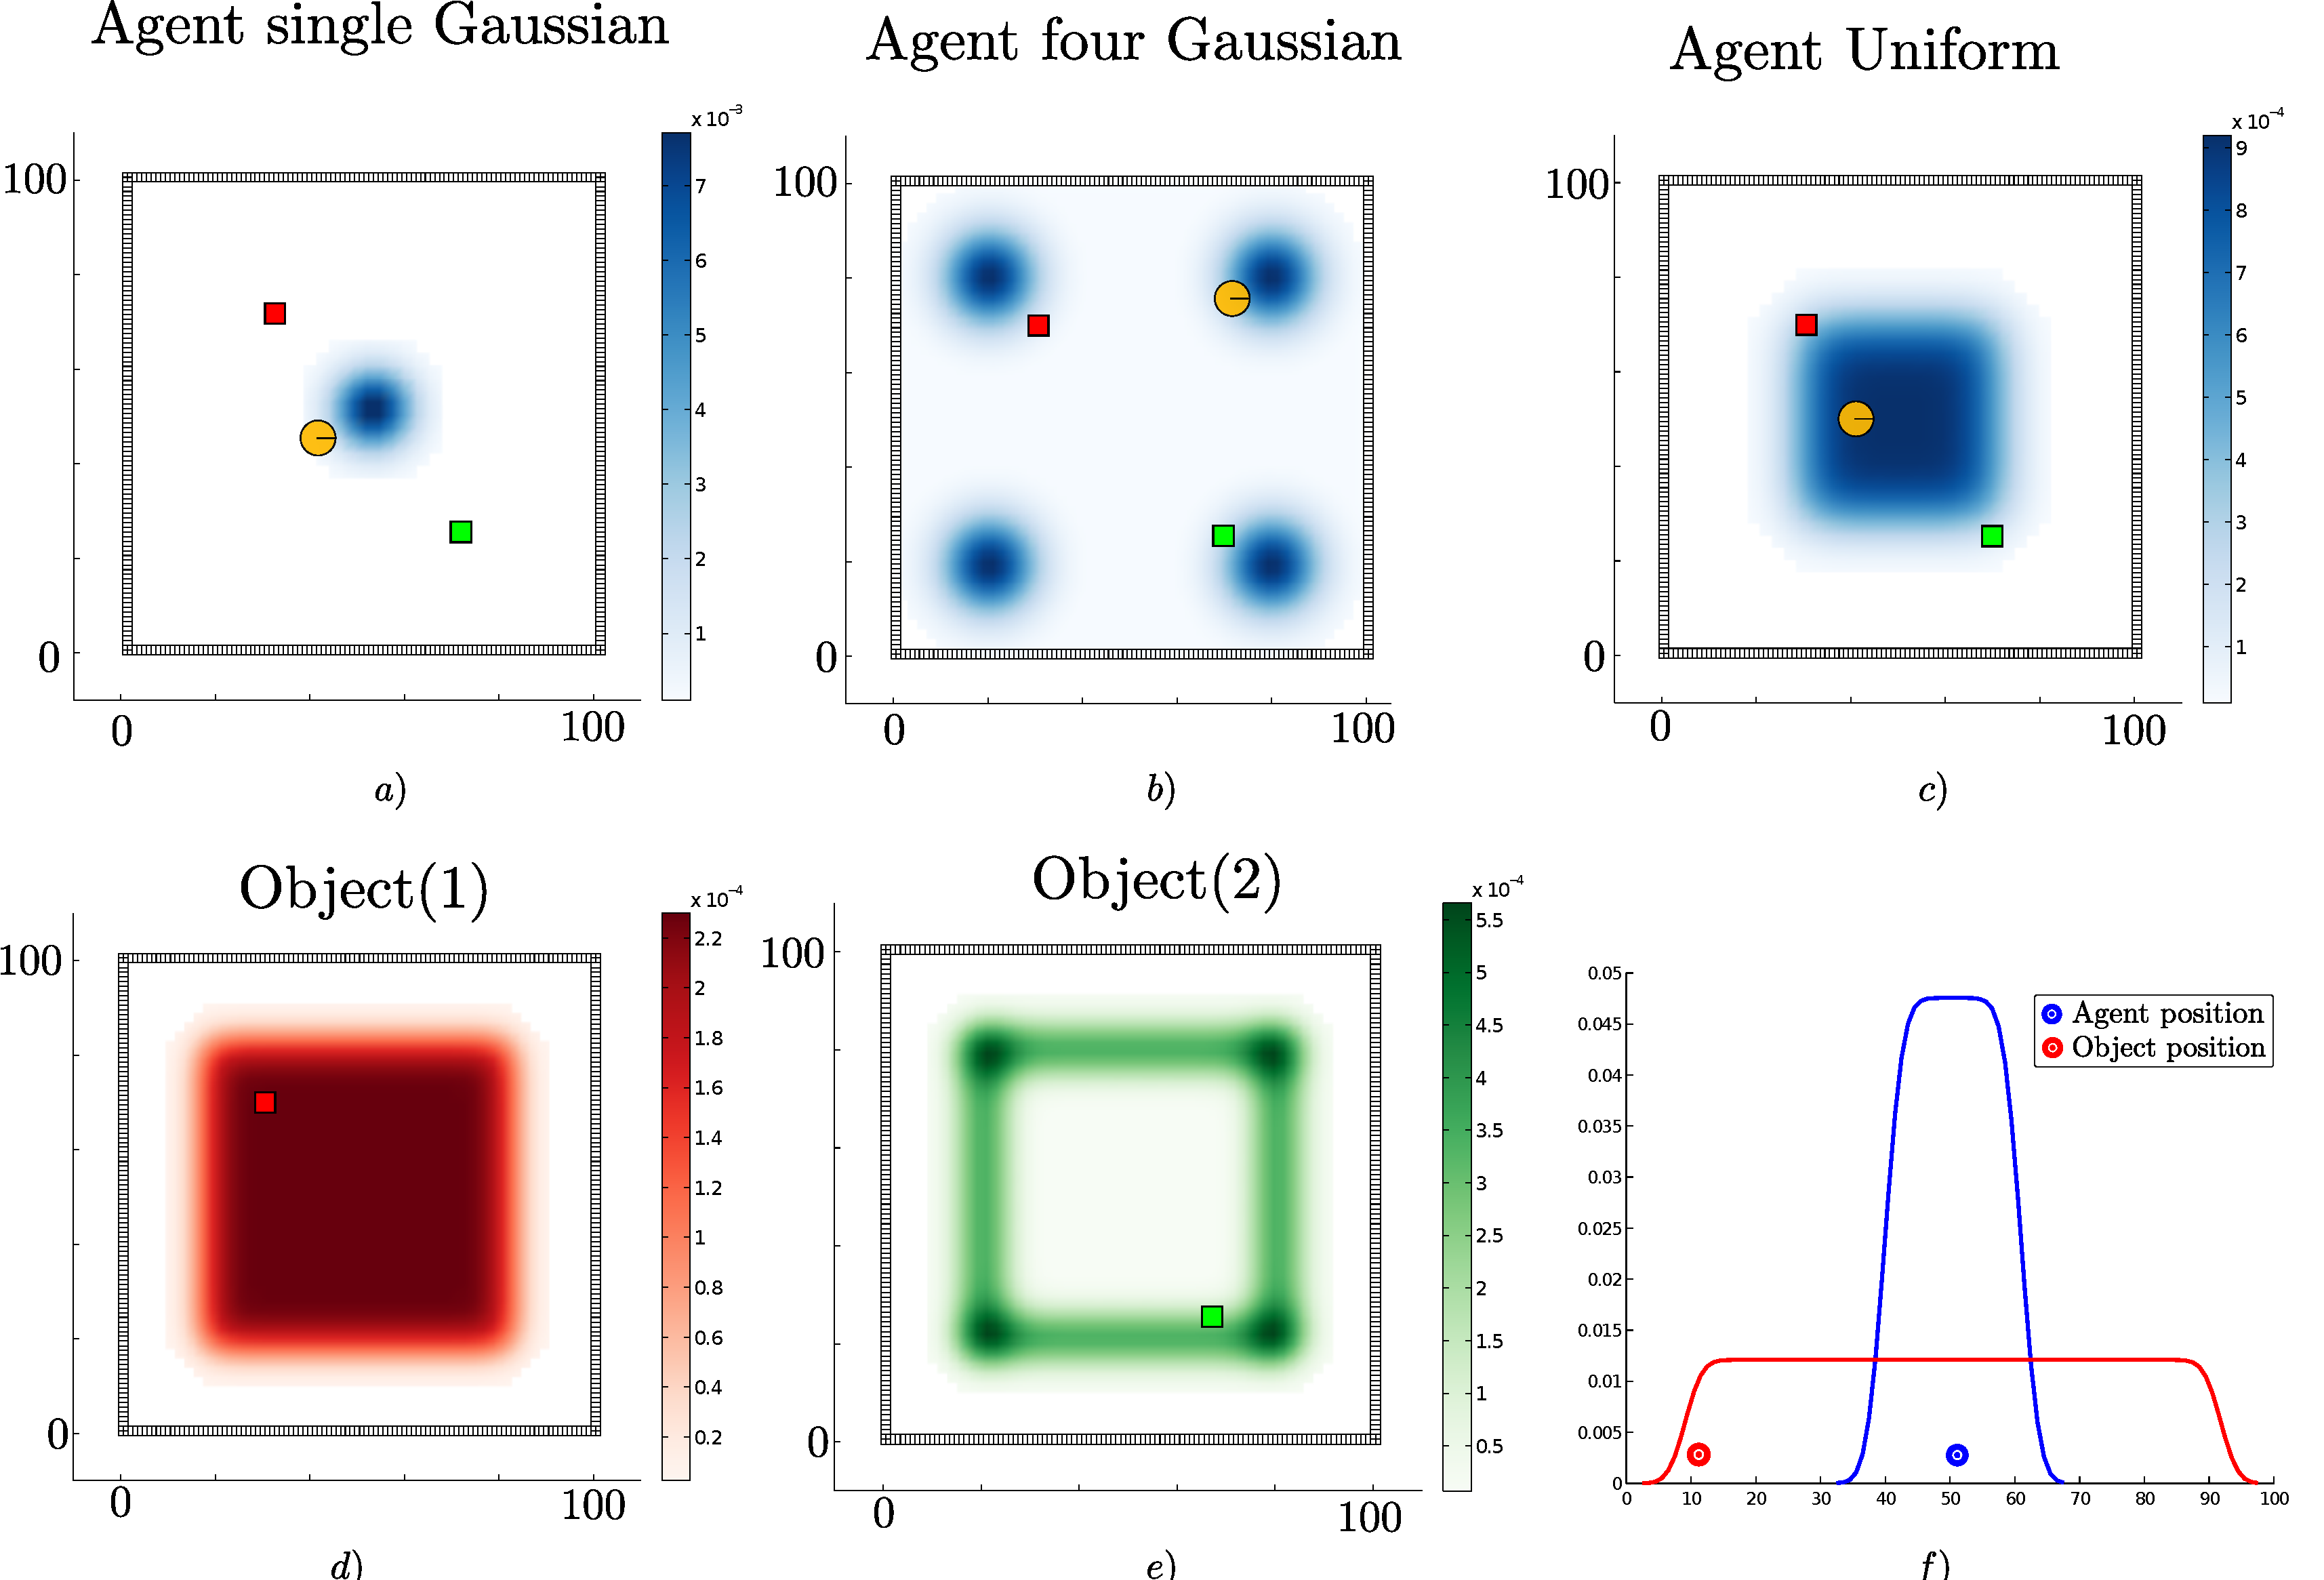
\includegraphics[width=\textwidth]{Figure14.pdf}
  \caption{\textbf{Agent's prior beliefs.} Two types of environment, the first is 
  a 2D world in which the agent lives in a square surrounded by a wall whilst the second is a 1D
  world. In the 2D figures the agent is illustrated by a circle with a bar to indicate its heading. The true location 
  of the objects are represented by colour coded squares. \textit{Top row} three different initialisations of the agent's location. 
  \textit{Bottom row} d) the agent's prior beliefs with respect to the location of the first object and e) belief of the second object's location.
  \textit{bottom row} f) 1D world with one object.}
  \label{fig:exploration_init}
\end{figure}

For the 2D search we consider three different initialisations (single-Gaussian, four-Gaussian, Uniform) for the agent's belief where there are 
two objects to be found. Ten searches were carried out for each of the three initialisations of the agent's beliefs. 
The true location of the agent, for each search, is sampled from its initial belief and the objects' locations 
(red and green squares in Figure \ref{fig:exploration_init}) are kept fixed throughout all searches. We repeat each search for 18 different memory 
sizes going from 1 to $N$ (the number of states). For the 1D search case we consider 1 object since adding more objects will make the search easier. 
We are interested in how the memory effects the search and not the search itself. In Figure \ref{fig:time_to_reach_goal} we report on the time taken to 
find all objects with respect to a given memory size which is shown as the percentage of the total number of states. 
In the 1D search case the variability of time taken to find the object converges when the memory size is at 60\% of the original state space. 
As for the 2D search with 2 beliefs (agent \& 1 object) the convergence depends on the agent's initial belief. For the 1-Gaussian (green line) 
all searches take approximately the same amount of time after a memory size of 9\%. As for the remaining two initialisations convergence is achieved at  48\%. 
The same holds true for the case of 3 beliefs (agent \& 2 objects).

In the 2D searches, the size of the memory has a less drastic impact than in the 1D (which is a special search case). 
In the 2D case only when the memory size is less than 6\% is there a significant impact in terms of the time taken to find 
the objects. We conclude that at least in the case of the greedy one step-look ahead planner which is frequently used in the literature, the 
size of the memory seems not to be a limiting factor in terms of the time taken to accomplish the search.


\begin{figure}
  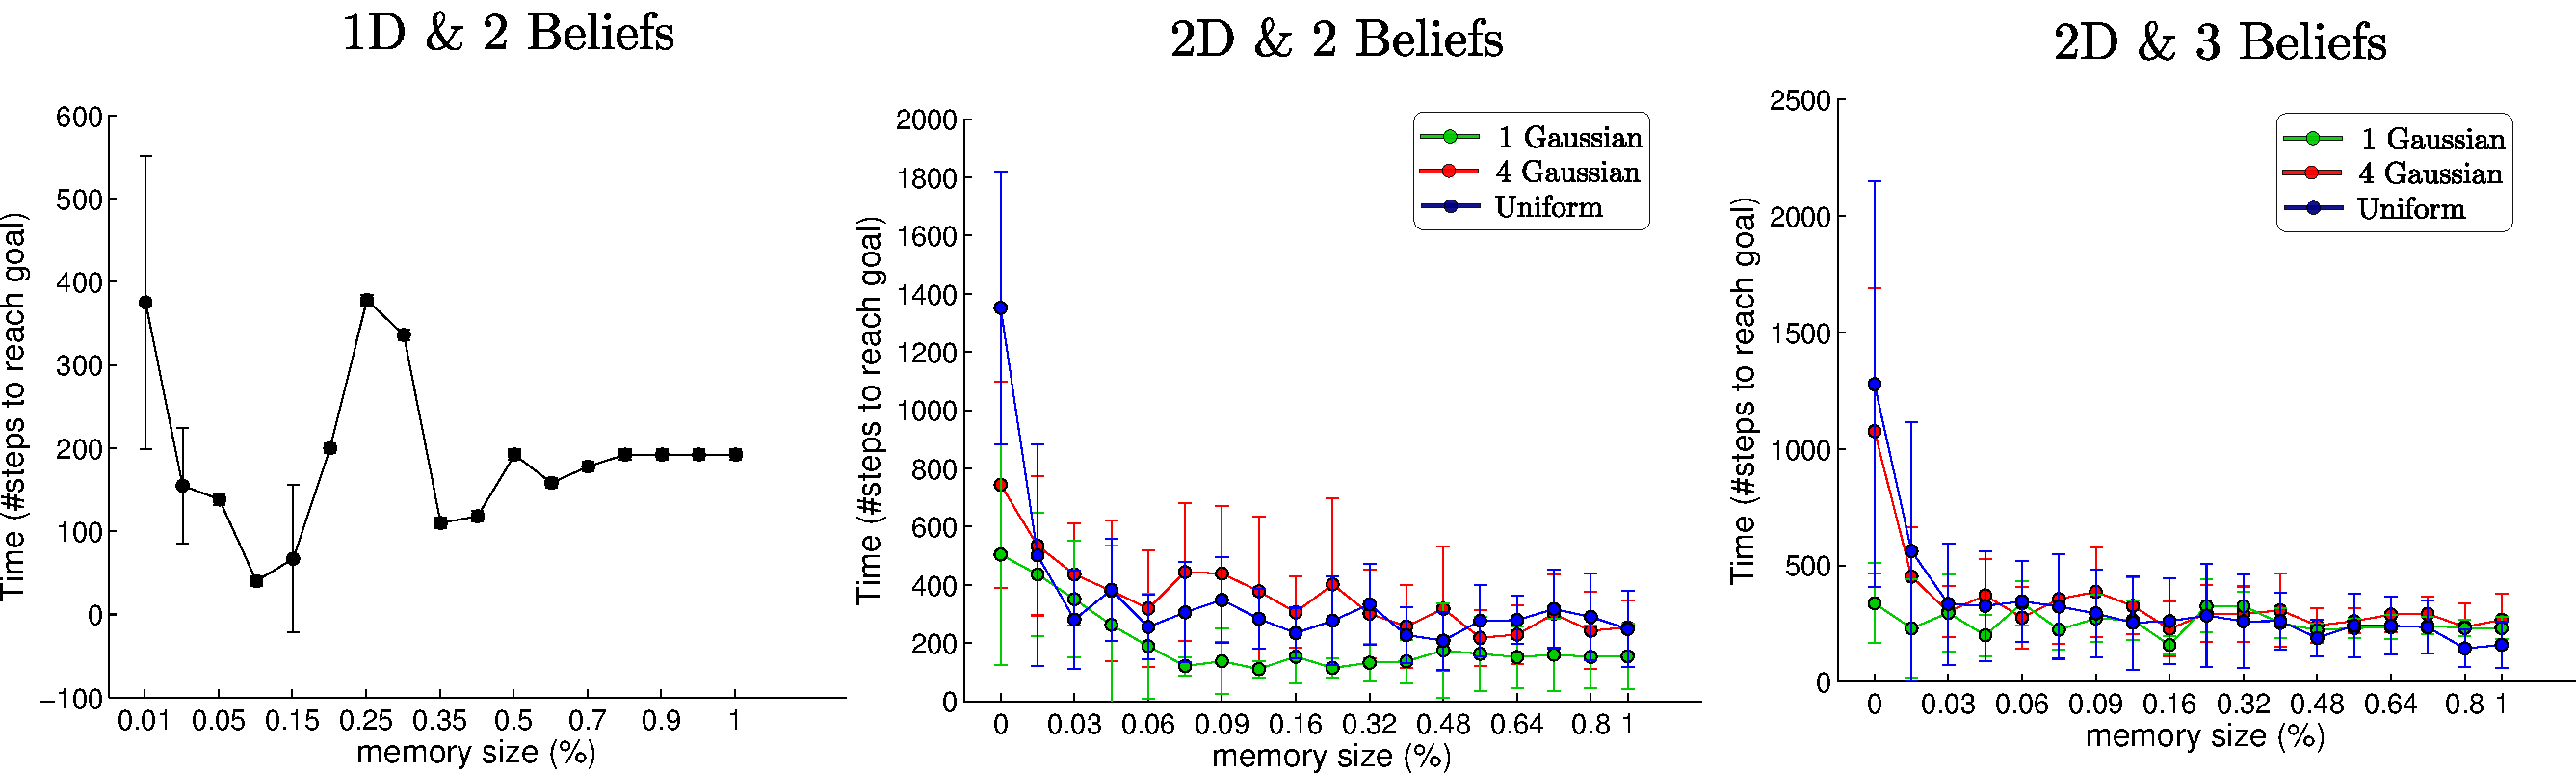
\includegraphics[width=\textwidth]{Figure15.pdf}
  \caption{\textbf{Memory size vs time to find objects} Results of the effect of the memory size on the decision process.
  The memory size is reported as the percentage of total number of states present in the marginal space. At 100\% the size
  of the memory is equal to that of the state space. \textit{left:} results of the 1D search illustrated in Figure \ref{fig:exploration_init} \textit{f)}.
  \textit{Middle \& right:} 2D search with initialisations accordingly depicted in Figure \ref{fig:exploration_init}.
  }
  \label{fig:time_to_reach_goal}
\end{figure}

\FloatBarrier
\section{Conclusion}

This work addresses the Active-SLAM filtering problem for scenarios in which sensory information relating to the map is very limited. Current
SLAM algorithms filter the errors originating from sensory measurements and not prior uncertainty. By making the assumption
that the joint distribution of all the random variables is a multivariate Gaussian, inference is tractable. Since the origin of 
our uncertainty is not originating from the measurement noise we cannot assume the joint distribution to have any special structure. 
A suitable filter for such purposes is the histogram which makes no assumption about the shape or form the joint distribution might take. 
The drawback of this form of parametrisation is that the space and time complexity is exponential with respect to the number of states and random variables 
and is a major limiting factor for scalability. 

The main contribution of this work is a formulation of a histogram Bayesian state space estimator in which the computational complexity is 
both linear in time and space. We took a different approach to other SLAM formulations in the sense that we did not
explicitly parametrise the joint distribution but kept all parametrisation in the space of the marginals (beliefs),
avoiding the exponential increase in parameter space which would otherwise have been the case. Our filter's parameters 
consist of the marginals and the history of measurement functions which have been applied. By evaluating the joint 
distribution solely at the states which are affected by the current measurement function whilst taking into account the 
memory, the MLMF filter can recover exactly the same filtered marginals as the histogram filter. The worst case space complexity is 
linear rather than exponential and the time complexity remains exponential but grows at a slower rate than in the histogram filter.
In the striving to make the filter scalable we introduced an independence assumption between the objects. An individual MLMF filter
was used for each agent-object pair. We evaluated the difference between the scalable-MLMF filter with a ground truth provided 
by the histogram filter for 100 different searches with respect to the Hellinger distance between them. We concluded that 
the divergence was relatively small and thus the scalable-MLMF filter provides a good approximation to the true filtered
marginals. We evaluated the time taken to perform a motion-update loop for different discretisation of the state space (100 to 10'000'000 states) and 
number of objects (2 to 25) present. In most of the cases we achieved an update cycle rate below 1Hz. We evaluated how the increase of the number of states 
effected the computational cost. The relationship was found to be linear and thus is in agreement with our analysis of the asymptotic growth rate. 
We analysed the effect the memory size (the remembered number of measurement likelihood functions) has on the decision theoretic process of reducing
the uncertainty of the map and agent during a search task. We found that in the 2D case the memory size has much less of an effect that in the 1D case
and we conclude that it is unnecessary to remember every single measurement function.

The implications of the MLMF and scalable-MLMF filter is that we have a computationally tractable means of 
performing SLAM in a case scenario where a lot of negative information is present and  we cannot assume the 
joint distribution has any specific structure. The filter can be used at higher cognitive level than 
processing raw sensory information as it is often in Active-SLAM. It would be well suited for reasoning about belief 
of location of objects in a setting where the robot's field of view is limited.

An interesting future extension is to make the original MLMF filter scalable without introducing assumptions.
One possibility would be to consider Monte Carlo integration methods for inference. These can scale well to high dimensional 
spaces whilst still providing reliable estimates. A second aspect would be to investigate the possibility
of using Gaussian Mixtures as a form of parametrisation of the marginals so that it might be possible to blend our filter with  
EKF-SLAM. This would allow the parameters to grow quadratically with respect to the dimension of the marginal space as opposed to
exponentially as it is in the case with the histogram and MLMF filters.



\section{Appendix}

\subsection{Bayesian filtering recursion}\label{appendix:bayes_recursion}

\begin{align}
  P(A_t,O,Y_{0:t},u_{0:t}) &= \sum_{A_{t-1}} P(A_t,A_{t-1},O,Y_t,Y_{0:t-1},u_{t},u_{0:t-1}) \label{eq:br_chain} \\
		           &= \sum_{A_{t-1}} P(Y_t|\Ccancel[red]{Y_{0:t-1}},A_t,\cancel{A_{t-1}},O,\cancel{u_{t}},\cancel{u_{0:t-1}}) \label{eq:cancellations}
		           \cdot  P(A_t|A_{t-1},O,u_{t},\cancel{Y_{0:t-1}},\cancel{u_{0:t-1}}) \\\nonumber 
		           & \;\;\;\;\;\;  \cdot  P( A_{t-1},O,\Ccancel[red]{u_t},Y_{0:t-1},u_{0:t-1}) \\
		           &= \sum_{A_{t-1}} P(Y_t|A_{t},O) \cdot P(A_t|A_{t-1},u_{t}) \cdot P(A_{t-1},O,Y_{0:t-1},u_{0:t-1}) \\
		           &= P(Y_t|A_{t},O) \cdot \underbrace{\sum_{A_{t-1}} P(A_t|A_{t-1},u_t) \cdot P(A_{t-1},O,Y_{0:t-1},u_{0:t-1})}_{P(A_t,O,Y_{0:t-1},u_{0:t})}
\end{align}
From line \ref{eq:br_chain} to \ref{eq:cancellations} we apply the chain rule of probabilities.
All the cancellations on line \ref{eq:cancellations} come from the \textit{Markov Assumption} and the structure of the Bayesian network.
The resulting final Bayesian recursion is obtained by conditioning on the measurement and actions, which is the normalisation factor.

\begin{align}
 P(A_t,O|Y_{0:t},u_{0:t}) = \frac{P(Y_t|A_{t},O) \cdot P(A_{t},O|Y_{0:t-1},u_{0:t})}{P(Y_t|Y_{0:t-1})}
\end{align}


\subsection{Derivation of the evidence}\label{appendix:evidence}

From first principle, Equation \ref{eq:marginal_likelihood_memory}, we demonstrated that the marginal likelihood is simply the difference
in the probability mass located inside the measurement functions after applying $P(Y_t|A_t,O)$.

\begin{align} \label{eq:marginal_likelihood_memory}
 P(Y_t|Y_{0:t-1}) &= \sum\limits_{A_t}\sum\limits_{O} P(Y_t|A_t,O)\cdot P(A_t,O|Y_{0:t-1}) \\
		  &= \sum\limits_{A_t}\sum\limits_{O} P(Y_t|A_t,O)\cdot \Big(P_{\ominus}(A_t,O|{\color{red}Y_{0:t-1}}) + P_{\cap}(A_t,O|Y_{0:t-1})\Big)\\
		  &= \sum\limits_{A_t}\sum\limits_{O} P_{\ominus}(A_t,O|{\color{red}Y_{0:t}}) + P(Y_t|A_t,O)\cdot P_{\cap}(A_t,O|Y_{0:t-1}) \label{eq:marginal_likelihood_memory_last}
\end{align}

We use the fact that after applying the measurement likelihood function, which lies in the interval $0 \leq P(Y_t|A_t,O) \leq 1$, 
to the joint distribution, its sum will always be smaller than $1$.

\begin{align}
  \sum\limits_{A_t}\sum\limits_{O} P(Y_t|A_t,O) \cdot P(A_t,O|Y_{0:t-1})  &\leq \sum\limits_{A_t}\sum\limits_{O} P(A_t,O|Y_{0:t-1}) \\
  \sum\limits_{A_t}\sum\limits_{O} P(Y_t|A_t,O) \cdot P(A_t,O|Y_{0:t-1}) &\leq 1 \\
  P(Y_t|Y_{0:t-1}) &\leq 1 \\
  P(Y_t|Y_{0:t-1}) + \alpha &= 1 \label{eq:marginal_likelihood_equal_I}
\end{align}

We equate Equation \ref{eq:marginal_likelihood_equal_I} with \ref{eq:marginal_likelihood_memory_last} and find a solution for the marginal likelihood which
only depends on areas of the joint distribution which are dependent.
		   
\begin{align}		  
 \sum\limits_{A_t}\sum\limits_{O} P(A_t,O|Y_{0:t-1}) - \alpha  &= \sum\limits_{A_t}\sum\limits_{O} P_{\ominus}(A_t,O|Y_{0:t}) + P(Y_t|A_t,O)\cdot P_{\cap}(A_t,O|Y_{0:t-1}) \\
   \alpha &= \sum\limits_{A_t}\sum\limits_{O}  P_{\ominus}(A_t,O|Y_{0:t}) + P_{\cap}(A_t,O|Y_{0:t-1})\\
     & - P_{\ominus}(A_t,O|Y_{0:t}) - P(Y_t|A_t,O)\cdot P_{\cap}(A_t,O|Y_{0:t-1}) \\
    \alpha &= \sum\limits_{A_t}\sum\limits_{O} P_{\cap}(A_t,O|Y_{0:t-1}) - P(Y_t|A_t,O)\cdot P_{\cap}(A_t,O|Y_{0:t-1}) \label{eq:marginal_likelihood_equal_I2}
\end{align}

The last line, Equation \ref{eq:marginal_likelihood_equal_I2}, when substituted back into line \ref{eq:marginal_likelihood_equal_I}, tells us that the normalisation factor or marginal likelihood is $1$ minus the difference in the area of
dependence a priori to the application of the measurement function.

\subsection{Derivation of the marginal}\label{appendix:marginal}

The marginal of a particular random variable is the marginalisation or integration over all other random variables, $P(A_t,|Y_{0:t}) = \sum\limits_{O} P(A_t,O|Y_{0:t})$. Below 
we give a form of this integration which exploits the independent regions in the joint distribution.
\begin{align}
 P(A_t,|Y_{0:t}) &= P(A_t|Y_{0:t-1}) - \Big(P(A_t|Y_{0:t-1}) - P(A_t|Y_{0:t}) \Big)  \\ 
		  &=  P(A_t|Y_{0:t-1}) - \Big(P_{\cap}(A_t|Y_{0:t-1}) + P_{\ominus}(A_t|Y_{0:t-1}) -  P_{\cap}(A_t|Y_{0:t}) + P_{\ominus}(A_t|Y_{0:t})   \Big) \label{eq:dependence1} \\
		  &=  P(A_t|Y_{0:t-1}) - \Big(P_{\cap}(A_t|Y_{0:t-1}) -  P_{\cap}(A_t|Y_{0:t})  \Big) \label{eq:dependence2} 
\end{align}


\subsection{Space \& time complexity (scalable-MLMF)}\label{appendix:space_time_scalable_mlmf}


\subsection{Space complexity}

\paragraph{Scalable-MLMF}
The initial number of parameters is $\left(M - 1\right) \cdot \left(2 \cdot (2 \cdot N)\right)$. The $(2 \cdot N)$ is the cost per random variable
as before, the additional factor of $2$ arises because we model pair-wise joint distributions and there are two random variables per joint distribution. The final
factor $\left(M - 1\right)$ corresponds to the total number of joint distributions, in the case of $M$ random variables. The final cost is then 
$(M - 1) \cdot N \cdot \left(4 + D\right)$ when taking into account the history.

\subsection{Time complexity}

\paragraph{Scalabe-MLMF} The computational cost is $\BigO{2 \cdot \left(M - 1\right) \cdot N }$. For one agent-object joint distribution, $N$
states lie in the area of influence of the measurement function. Given $M$ random variables, the number of states needed to evaluate in all the joint distributions
is $M-1$. The final marginal of the agent $P(A_t|Y_t) = \prod\limits_{i=1}^{M-1} P(A^{(i)}_t|Y^{(i)}_t)$ is obtained through $(M-1)\cdot N$ multiplications or additions.
This explains the factor of $2$ in the final computational cost.

\paragraph{Memory}\label{appendix:memory_time_complexity}

The MLMF filter stores the history of all likelihood functions which have been applied on the joint distribution. This is the 
memory term $P(Y_{0:t-1}|A_t,O)$ in Equation \ref{eq:joint_filter_memory}. Table \ref{tab:memory_list} shows the memory list after three 
iterations and the resulting effect in  the joint distribution is illustrated in Figure \ref{fig:3bel_lik_profile} \textit{right}.

\begin{table}
\begin{center}
 \begin{tabular}{llc}
 $P(Y_{0 }|A_0,O)  = $  & $P(Y_0|A_0,O)$				                            & (t=0) \\
 $P(Y_{0:1}|A_1,O) = $  & $P(Y_1|A_1,O) \cdot P(Y_0|A_1,O+u_1)$                             & (t=1) \\
 $P(Y_{0:2}|A_2,O) = $  & $P(Y_2|A_2,O) \cdot P(Y_1|A_2,O+u_1) \cdot P(Y_0|A_2,O+u_1+u_2)$  & (t=2)
\end{tabular}
\end{center}
\caption{\textbf{Memory list} After three updates the memory term $P(Y_{0:t}|A_t,O)$ contains three functions. The parametrisation
of the functions is the same with the exception of actions $u_t$ which are added after each motion update step. As the result the 
first function added to the list will have all the actions applied to it from the first time step to the last.}
\label{tab:memory_list}
\end{table}

At every time step the current action (causing a displacement) is applied to all elements in the memory before appending the new 
measurement function $P(Y_t|A_t,O)$. The application of the actions causes a shift of likelihood functions along the agent's axis
in the joint distribution. As a result, the memory list is always sorted and the first element is always the last measurement function
to have been applied. 
During the measurement update Equation \ref{eq:marignal_mrf_2}, only the first entry of the memory function has to be evaluated
giving a cost of $\BigO{1}$ at every time step when evaluating the dependent states (those which lie on the hyperplane). When
evaluating a point which is not on the hyperplanes, its offset ($c$) can be evaluated $A=O+c$ and checked whether it is contained
within the list. We employ a binary search which has a time complexity of $\BigO{\log(n)}$ (where $n$ is the current size of the memory). This is not necessary during most
of the filtering process since the dependent states to be evaluated in the joint distribution always lie on the line $A=O$.

\section*{References}

\bibliography{citations}

\end{document}

